\documentclass{UCreport} 



\usepackage[authoryear,comma,round]{natbib}
\usepackage{hyperref,graphicx}
\usepackage[separate-uncertainty=true,multi-part-units=single]{siunitx}

\usepackage{caption}
\usepackage[list=true,listformat=simple]{subcaption}
\makeatletter
\g@addto@macro\p@subfigure{.}
\makeatother

% \usepackage[margin=1.5cm, left=3cm ,twoside]{geometry}

\usepackage[para]{footmisc}

\usepackage[super]{nth}

\usepackage{amsmath,amssymb}

\DeclareSIUnit{\arcsec}{''}
\DeclareSIUnit{\au}{\mathrm{AU}}
\DeclareSIUnit{\mag}{\mathrm{mag}}
\DeclareSIUnit{\px}{\mathrm{px}}

\usepackage[utf8]{inputenc}
\usepackage[T1]{fontenc}
\usepackage{newunicodechar}

\DeclareRobustCommand{\okina}{%
  \raisebox{\dimexpr\fontcharht\font`A-\height}{%
    \scalebox{0.8}{`}%
  }%
}
\newunicodechar{ʻ}{\okina}
\newcommand{\omuamua}{\okina Oumuamua }


% \title{ASTR480 Final Report:\\
% \textit{Asteroids in TESS}
% }
% \author{Brayden Leicester \\ 
% \textit{61352063} \\
% [1ex]\small{Supervisors: Michele Bannister and Ryan Ridden-Harper}
% }
\begin{document}



%----------- Report information ---------

\logo{logos/UC.png}
\school{\textbf{School of Physical and Chemical Sciences}}
\course{\textbf{ASTR480}}
\student{\textbf{Brayden Leicester}}
\supervisor{Dr Michele Bannister and Dr Ryan Ridden-Harper}
\ttitle{Asteroids in TESS} %title of the file


%----------- Init -------------------

\buildmargins % display margins
\buildcover % create the front cover of the document



%------------ Declaration ----------------
\pagenumbering{roman}
\addcontentsline{toc}{section}{Declaration}
\declaration

I certify that content of this report was mostly my own work.
\\

My supervisors helped by proofreading the report and offering feedback. As well as providing useful insight into problems when I was stuck.\\

Graduate students, X and Y, helped me understand ... \\

The derivation in section 3 was taken from ... \\

\autoref{Fig:FreqVsDiam} has been recreated after data from the Light Curve Database (LCDB) \citet{Warner2009}, as cited in text. That data has been supplemented with my own work in the corresponding \autoref{Fig:FreqDiamUpdate}.

\vspace{2cm}
\begin{centering}
  \textbf{\student}\par
\end{centering}

\newpage

%------------ Abstract ----------------

\addcontentsline{toc}{section}{Abstract}
\abstract

This is where the abstract goes. \\

This is the next paragraph.

% %*Background

% %*Methods

% %*Main Results

% %*Conclusion

\newpage
%------------ Contents pages ----------------

\toc % creates the table of contents

\addcontentsline{toc}{section}{List of Figures}
\listoffigures
\newpage
\addcontentsline{toc}{section}{List of Tables}
\listoftables
\newpage

%------------ Report body ----------------
\pagenumbering{arabic}

\section{Introduction}\label{Sec:Intro}

%To get all asteroids in TESS. 
This project aims to find and characterise the light curves of all the asteroids seen by the Transiting Exoplanet Survey Satellite (TESS).
Combining knowledge of these asteroids positions with the high cadence imaging of TESS should allow for the determination of rotation periods of these small bodies, and the amplitude of the variation.


\subsection{Asteroids}\label{SubSec:Asteroid}

Asteroids are a key class of solar system objects. Much is known about them already, but there is always more to learn.
The orbits of asteroids can be well characterised by only a few values, the proper elements of the object.
These are the lenght of the long axis of elliptical orbit, the semi-major axis, $a$, how elliptical the orbit is, the eccentricity, $e$, and the angle to the ecliptic plane, the inclination,$i$.
Typical values for main belt asteroids are an $a$ of \qtyrange{2}{3.3}{\au}, an $e$ in \qtyrange{0}{0.35}{} and an $i$ around \qtyrange{0}{30}{\degree} \citep{DeMeo2015}.
Comets have undefined $a$ and larger $e$, with some long period comets having $e\approx 1$, but the typical range is \qtyrange{0.2}{0.7}{} \citep{Lewis2012}.
Interstellar objects (ISOs) have $e>1$ as they are on unbound hyperbolic trajectories \citep{McGlynn1989}.


% The semi-major axis, $a$, is the largest distance from the sun that the asteroid achieves on its elliptical orbit.
% Main belt asteroids have a typical $a$ of \qtyrange{2}{3.3}{\au} \citep{DeMeo2015}.
% The bounds between the inner, middle and outer main belt at \qty{2.5}{\au} and \qty{2.82}{\au}, these separations are due to resonances with Jupiter (the 3:1 and 5:2 mean motion resonances mark the edges of middle main belt) and Saturn (the $\nu_6$ secular resonance cuts off the lowest $a$ edge of the inner belt) carving swathes where asteroids cannot be in stable orbits.

% The eccentricity, $e$, of this orbit is the next proper element. $e=0$ implies a perfectly circular orbit, $0<e<1$ are ellipses, $e=1$ give a parabolic orbit, and $e>1$ are unbound, hyperbolic orbits.
% Main belt asteroids have small $e$, in the range of  \citep{DeMeo2015}
% Comets have larger $e$, with some long period comets having $e\approx 1$, but the typical range is \qtyrange{0.2}{0.7}{} \citep{Lewis2012}.
% Interstellar objects (ISOs) have $e>1$ as they are on unbound hyperbolic trajectories.

% The inclination, $i$, of asteroids is also a key orbital element, it is the angle relative to the ecliptic plane.
% In principle asteroids can span the whole range of inclinations, though they rarely do.
% Main belt asteroids have typical inclinations of \qtyrange{0}{30}{\degree} \citep{DeMeo2015}, so the TESS cameras closer to the ecliptic plane are expected to have the most asteroids in their fields.

Asteroids can be grouped into families based on clustering of the proper orbital elements and similarities in their colour or spectra \citep{Nesvorny2015}.
These families are named for their largest member.
Families are thought to all originate from the same body that was destroyed by a collision earlier in the solar system's history.

%TODO Rotation of asteroids
As an asteroid rotates, the amount of sunlight reflected changes with time.
This produces a lightcurve that is often sinusoidal in appearance.
These lightcurves are normally ``double-peaked'', having two maximums for one full rotation of the body, due to symmetries in the shape of the object.
The shape of the asteroid has a large effect on the scale of variation in the lightcurve \citep{Durech2015}, the more elongated the object is, the larger the variation.
The rate of rotation is limited by the size of the asteroid \citep{Pravec2000}, as the internal strength of the body is put under too much strain if large asteroid rotate with short periods.

Understanding the rotation properties of asteroids has long been of interest to astronomers \citep[e.g.][for early work into the limits of rotation period and the tumbling nature of some small bodies]{Weidenschilling1981,Harris1994}.
This is still at the forefront of research, with more lightcurves being published year-on-year \citep{Harris2015}.
For the smallest objects ingenious observation techniques are employed to measure rotation periods such as intentionally streaking the asteroid down a column of pixel on a detector, and making the lightcurve from the streak, as done by \citet{Bolin2023}.

Asteroids can have their rotation properties changed with time, collisions can do this, and so can light from the sun.
The YORP effect (named for the discoverers Yarkovsky, O'Keefe, Radzievskii, and Paddack) is the process of tourquing asteroids of an asymmetric shape by both bombardment of photons and thermal (re-)emission \citep{Rubincam2000}.

The data on solar system bodies will only increase with more large survey telescopes coming online soon, such as the Legacy Survey of Space and Time \citep[LSST][]{LSST2019}.
The number of new asteroids that are well characterised will increase by more than 2 orders of magnitude on the Sloan Digital Sky Survey \citep[SDSS][]{York2000} which had $\sim 88000$ objects \citet{Parker2008}.
LSST needs a dedicated pipeline for asteroid classification, the Solar System Notification Alert Processing System \citep[SNAPS][]{Trilling2023} has been developed using Zwicky Transient Facility \citep[ZTF, ][]{Bellm2018} data and can scale up handle volume of data coming from LSST.
Work is being done to understand the biases of how  asymmetric shape high amplitude variations can lead to selection effects of such large sample of asteroids \citet{Levine2023}.

Because of such a rich history of study, many asteroids have a known rotation period.
These are catalogued by \citet{Warner2009} in the Light Curve Database (LCDB).
In the October \nth{1}, 2023 release, the LCDB has nearly 9000 objects with periods determined to a quality code $U\geq 2-$, which is the minimum reliability recommended by \citeauthor{Warner2009} for statistical analysis.
This includes other TESS data from \citet{Pal2020} and \citet{Woods2021}.
The frequencies against diameter plot of these asteroids in \autoref{Fig:FreqVsDiam} shows the collection of all the asteroids in the LCDB with $U\geq 2-$.
The diameter presented in the LCDB here calculated from the absolute magnitude $H$ of the bodies, assuming an albedo.
\citeauthor{Warner2009} acknowledge that there are direct measurements of diameter for more asteroids in the present day, but continue to present the $H$ derived diameters for consistency.

The asteroid spin barrier \citep{Pravec2000} is seen in the red dashed lines in \autoref{Fig:FreqVsDiam}.
There are very few asteroids larger than $\qty{0.15}{\kilo\metre}$ rotating faster than $\sim \qty{10}{\per\day}$.
It is thought that the YORP effect, as well as collisions, spin up asteroids so fast that they pass above this barrier and then no longer have the internal strength necessary to hold themselves together.
This implies that all asteroids made to spin faster have torn themselves apart and that they have no tensile strength, i.e they are rubble piles instead of monoliths \citep{Harris1996}.
This idea of the cohesive strength of small bodies is still explored today \citep[e.g.][for V-type asteroids]{Oszkiewicz2020}.

Comparing the periods I calculate of asteroids that are already in the LCDB is key to making sure my methods are reliable, and that the periods for asteroids for which no data exists can be trusted.

\begin{figure}[h]
  \centering
  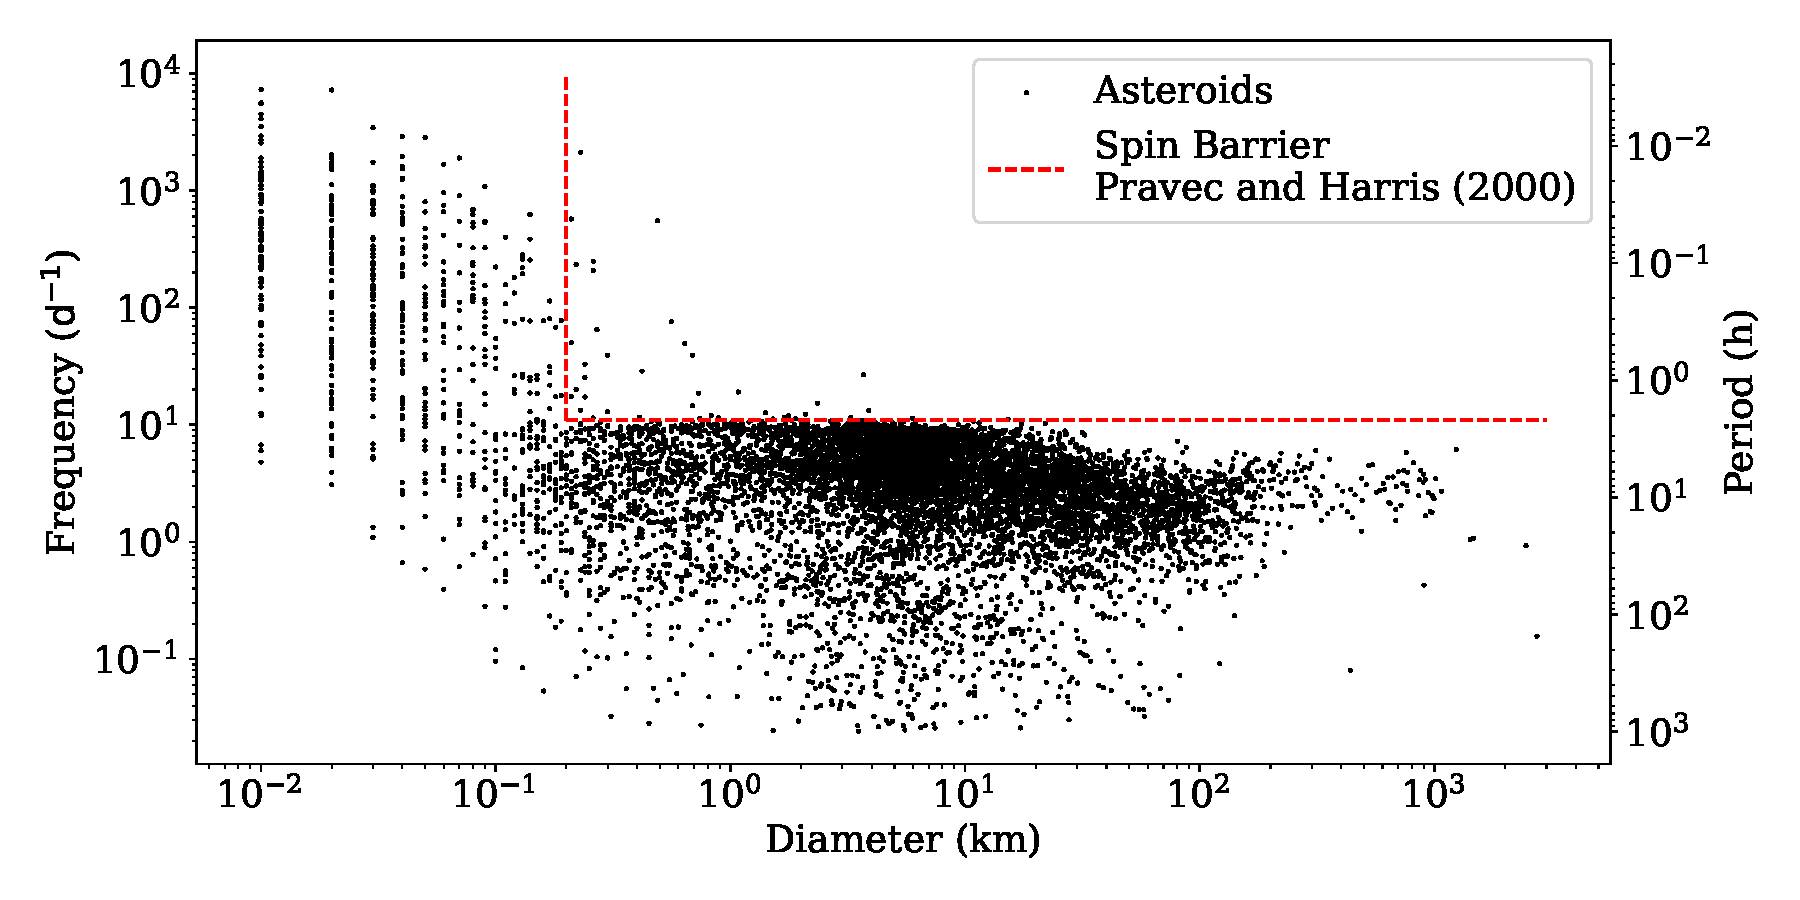
\includegraphics[width=0.7\textwidth]{./Figures/Diam-FreqPlot.pdf}
  \caption[Asteroid frequencies vs diameter (LCDB)]{
    Rotation rate of asteroids by their size, recreated from the  October \nth{1}, 2023 LCDB after \citet{Warner2009}.
  }
  \label{Fig:FreqVsDiam}
\end{figure}

\subsubsection*{Interstellar Objects}
%Omuamu
High amplitude variation has come to the forefront of questions about asteroid properties because of the first interstellar object, 1I/\omuamua \citep[see][for a review]{Bannister2019}.
\omuamua was determined to be spectroscopically red \citep{Fitzsimmons2017, Meech2017}, and having a photometric colour in the neutral end of the solar system range \citep{Bannister2017}.
1I was classed as asteroid due to lack of a coma, and no noticeable activity.
This contrasts the second ISO, 2I/Borisov, which had many cometary characteristics \citep[see ][for a review]{Dorofeeva2023}.

\omuamua was measured to have a rotation period of \qty{8.67(0.34)}{\hour} \citep{Belton2018} and seemed to be tumbling \citep[e.g.][]{Drahus2018,Fraser2018}.
Combing the tumbling with an elongation ratio of up to \qty{6(1)}{}:1 \citep{McNeill2018}, 1I is said to have a cigar shape \citep{Belton2018}.
The peak to peak amplitude variation of this ISO was \qty{2.5}{\mag} \citep{Meech2017} over its double-peaked lightcurve, which is interesting as it is more variation than most asteroids more than most asteroids \citep[as seen in the LCDB of][]{Warner2009}.
With the full sky survey of bright asteroids, I hope to and to see just how rare \omuamua is, by finding many asteroids with large amplitude variations.


\subsection{TESS}\label{SubSec:TESS}

%Why TESS
TESS is a large area, high cadence imaging, space telescope  \citep{Ricker2014}.
TESS is tasked with observing one piece of sky for \qty{27}{\day} at a time , which defines a sector.
The telescope delivers \qtyproduct{96 x 24}{\degree} full frame images (FFIs) at regular intervals.
These FFIs are built from stacked \qty{2}{\second} exposures, leveraging the short readout times of the 16 charged-coupled devices (CCD) spread over four cameras on-board.
With the initial cadence for these full frame images set to \qty{30}{\minute}, the time resolution of TESS is unparalleled.
As the mission was extended, after TESS had already mapped the entire sky, the length of the FFIs has decreased to \qty{10}{\minute} and then later to \qty{200}{\second}.
This high time resolution and observation area does come at the cost of spatial resolution, as the pixels are each \qty{21}{\arcsec} square.

Of interest here is what such a high sampling rate can do for statistics on the asteroid population.
For bright asteroids the rotation periods should be able to be easily determined from this vast dataset, due to the high sampling of the lightcurve.
The shortest FFIs will be able to accurately determine the rotation periods of all but the fastest rotating asteroids, most of which will be too dim to see in the TESS data.

The highest frequency (shortest period) that can be found from time series data like this is at the Nyquist limit, twice the minimum time between images.
Due to the short cadence, the Nyquist frequency of TESS is quite high, \qty{1}{\per\hour}.
This is well sampled enough to characterise most variable stars, as well as find the orbital periods of exoplanets to a high precision.
The decreased in the FFI exposure time in later sectors comes with a complementary increase in the Nyquist frequency.

Previous work has been conducted to find and classify all the asteroids in TESS data.
\citet{Pal2018} proposes that TESS will be a good instrument for solar system object study, and simulate some detections down to \nth{20} visual magnitude, but that good photometry should only be expected to $V \lesssim 19$, a sentiment shared by \citet{Wong2019}.
The first data release in \citet{Pal2020} catalogues nearly 10,000 asteroid light curves from the first year of TESS operation, and they report that they triple the number of asteroids with accurate rotation periods.
\citet{McNeill2023} also analyse TESS cycle 1, and detect almost 38,000 objects.
They determine reliable rotation periods for about 3,500 asteroids in this sample and show a lack of reliability for objects with periods less than \qty{3}{\hour}.
In the overlap from the data from \citet{Pal2020}, \citeauthor{McNeill2023} find good agreement between the two sets of periods and amplitudes.
The Minor Planet Center (MPC) gets regular updates from TESS thanks to the work of \citet{Woods2021} and their \texttt{LINEAR-TESS} program, which creates tracklets of objects over a day, and then stitches these together to form a track of each asteroid through an FFI.

There is ongoing analysis of subsets of the asteroid population in TESS.
\citet{Gowanlock2024} uses TESS photometry as well as  observations by ZTF to get a longer baseline on mutually observed objects while combining ground and space based observations.
There were not very many objects in both samples with known periods for comparison, with only 222 objects analysed, however they demonstrate that the technique is effective.
Fainter and unknown solar system objects can be found by shift and stacking \citep{Holman2019, Payne2019,Rice2020} or taking a fast X-ray transform \citep{Nguyen2024} of the FFI data.

This work aims to extend these studies to more sectors, hence characterising more asteroids.
The goal is to get a volume complete set of asteroid lightcurves and periods, by analysis of the whole sky as seen by TESS using data from more than just the first year of TESS's operation.
This has not been achieved, as the analysis of only one sector is presented here, but the methods are scalable.
Because of the survey properties, TESS provides a self-consistent way to measure the properties of asteroids over the full sky.
By using the higher cadence FFIs of later TESS sectors, the $P\leq\qty{3}{\hour}$ limit on the accurate periods \citep[as found by ][]{McNeill2023} can be lowered.
I also employ a different data reduction method, using reduced data from the \texttt{TESSreduce} package \citep{Ridden-Harper2021}.
This should increase the accuracy of the photometry due to the improved background subtraction process.


This work is part of a full sky transient survey using TESS, the TESS Extensive Lightcurve Logging and Analysis of Transient Events4 (\texttt{TESSELLATE}) pipeline \citep{TESSELLATE}.
To see what \texttt{TESSELLATE} detects and to help progress the pipeline, one can participate in the Cosmic Cataclysim Zooniverse project\footnote{\href{https://www.zooniverse.org/projects/cheerfuluser/cosmic-cataclysms}{https://www.zooniverse.org/projects/cheerfuluser/cosmic-cataclysms}}.
Asteroids can spike the brightness of a pixel for only a few frames while it is passing by.
This can confuse the pipeline looking for transients such as flare stars and supernova, as they can look very similar, having the brightness change in one pixel for a short time.
Knowing where the asteroids are will allow for the removal of these spikes from the transient pipeline, as well as to understand the asteroid population better.
By filtering the asteroid detections out, while also self consistently determining rotation properties of a large sample of the population, more science can be done with the one set of analyses.


\section{Methods}\label{Sec:Meth}

The \texttt{TESSELLATE} pipeline has been running on the OzSTAR supercomputing facilities.
I built this asteroid detection and subsequent lightcurve and periodogram analysis program by testing on one subsection of one CCD of one camera  of one TESS sector.
The code written can be accessed at my ASTR480 GitHub repo \footnote{\href{https://github.com/ble61/ASTR480}{https://github.com/ble61/ASTR480}}. 
Because of the large number of asteroids there are too many lightcurves to look at, so the code has to run with no human decisions. 
Once I was confident this worked as required, the same code was refactored slightly to work on OzSTAR and a large-scale analysis of a processed TESS sector was run.
% I will be looking for completeness of detections of asteroids, as well as accuracy of periods and amplitude variation.

For this work, I present analysis of TESS sector 29\footnote{\url{https://tess.mit.edu/observations/sector-29/}}, which was observed between \nth{26} August and \nth{22} September 2020.
This was the third TESS sector to be using \qty{10}{\min} cadence FFIs, which has had less analysis of the asteroids preformed.
It was chosen mainly because of this higher cadence, it was the only sector of this cadence that had been processed by \texttt{TESSELLATE} with enough time for my analysis to be preformed.
What is presented for this section is scalable, on a per-sector basis, to any sector that has been reduced.


\subsection{Querrying Databases for Asteroid Positions and Properties}\label{SubSec:Querry}

To check for asteroids in the TESS data, the positions of the asteroids with time are required.
For asteroids bright enough to be in TESS, their ephemeris is well known, so I needed to access their positions and then cross match them with transients in the TESS data.

\texttt{SkyBoT} \citep{Berthier2006} was queried to get positions of asteroids in a cone search.
A box in right ascension (RA) and  declination (Dec) space.
The search was limited to only asteroids with an average visual magnitude $V\geq \qty{20}{\mag}$.
As TESS sectors are \qty{27}{\day} long, so querying every \qty{12}{\hour} is both computationally feasible and allows for a good understanding of a bodies motion. 

These positions are still very sparsely spaced in time compared to the TESS data. 
An interpolation is needed to bridge the gap, this is preformed by \texttt{numpy} \citep{Harris2020}. 

Knowing where the asteroids are is helpful for finding them in the archival TESS data, but knowing more about the individual asteroids is also useful for population statistics.
The \texttt{astroquery} \citep{Ginsburg2019} package was used to query \texttt{JPL Horizons} was used to obtain the orbital elements of each asteroid, $a$, $e$, and $i$, as well as an absolute magnitude $H$, which is a good proxy for size (as discussed above). %TODO ref

\subsection{Interpolation of the Positions to Match TESS Cadence}\label{SubSec:Interp}


\begin{figure}[t!]
  \centering
  \includegraphics[width =0.8 \textwidth]{./Figures/interpPos\_29\_1\_2\_2.pdf}
  \caption[Interpolated Positions of Asteroids]{
    The interpolated positions of asteroids in one subsection of a TESS sector.
    The colours of the lines are time sequenced, as shown in the colour bar.
    The alpha of the colours are scaled by the absolute magnitude $H$ of the asteroid.
    Both celestial coordinates (RA and Dec) and ecliptic longitude and latitude  axes are shown.
    The green $+$ is the centre of the subsection.}
    \label{Fig:interpPos}
\end{figure}

  
\begin{figure}[t]
  \centering
  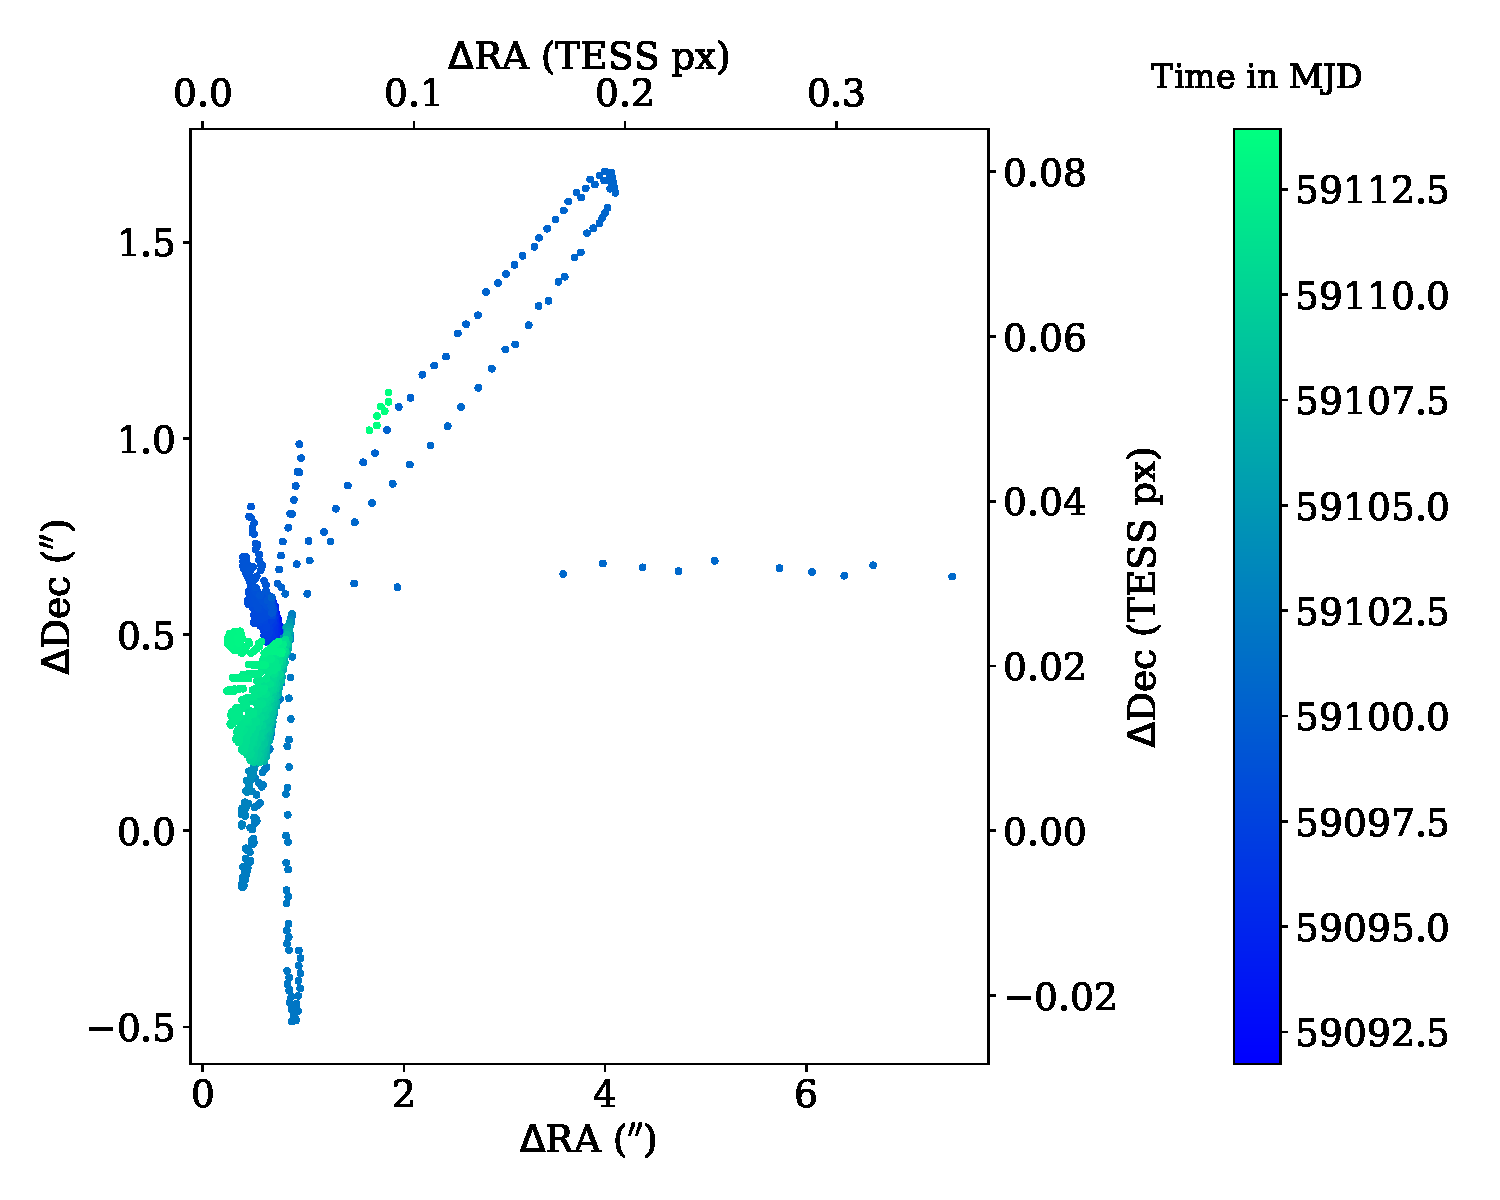
\includegraphics[width =0.8 \textwidth]{./Figures/1990 KC1PosCheck.pdf} %TODO one with more points???
  \caption[Interpolated Position Verification]{
  The difference in the interpolated position of an asteroid from queries to \texttt{JPL Horizons}. 
  The change in position in both arcseconds (\unit{\arcsec}) and TESS pixels are shown.  
  }\label{Fig:errPos}
\end{figure}

With TESS data coming in $\qty{10}{\minute}$ chunks, 72 interpolated points are needed between each API call.
A linear interpolation between the queried RA and Dec is preformed at the times of the TESS frames.
\texttt{TESSELLATE} saves out these time-frame pairs as part of its analysis, allowing for the time coordinate of any position to be exactly at a frame time.
This will also simplify the detection matching, as the any difference in the time will mean the detection is in a different frame. 

These interpolated positions can be seen in \autoref{Fig:interpPos} for a subsection of sector from \texttt{TESSELLATE}.
There are a few interesting features, such as the asteroids are moving in the same direction, indicated by the colouring, they come in from low RA and Dec and tend to increase both coordinates as the month of the sector progresses.
There is also a large size range in this slice of sky, ranging over \qty{5}{\mag} in absolute magnitude, which can be seen in the alpha (or transparency) of the tracks in \autoref{Fig:interpPos}.

Because of a small change in position between each frame, \citep[$\sim \qty{1}{\px}$ per \qty{30}{min} frame][]{Pal2018}, this interpolation should be accurate.
Checking against a higher frequency query to the \texttt{JPL Horizons} ephemeris  confirmed this accuracy on a few asteroids, as shown in \autoref{Fig:errPos}.
This is of asteroid ``(8654) 1990 KC1'', the largest difference is only a third of a TESS pixel in RA, so the interpolations are accurate enough for these measurements. 
All others checked are similarly accurate.
This is not a feasible way of getting all the positions, as the queries are per name and time, not per area and time like the cone search in \texttt{SkyBoT}.
They are also rate limited, so while a few asteroids can be checked, filling the gaps between the \texttt{SkyBoT} half day queries for all the asteroids would be too expensive.



\subsection{Matching Asteroids to \texttt{TESSELLATE} Detections}\label{SubSec:Match}

Matching these interpolated positions to \texttt{TESSELLATE} detections is important to lower the unknown transient outputs of this pipeline.
Having interpolated their positions, the asteroids have a well sampled set of RA, Dec and time values of where they should be in the TESS data.
They should show up in a single pixel in $xy$ space for a small number of frames, of order $\sim1$.
This is the same as a lot of other transient events, a sharp rise in brightness and then disappearing quickly again.
The number of frames for events is variable, type Ia supernova will brighten is a matter of a few hours and then dim for days, while stellar flares are of similar profile by a smaller max brightness and a correspondingly shorter decay time.

Asteroids are very short events, however these detection pipelines are robust and do pick them up.
These pipelines have already found the aforementioned supernova, stellar flares and variable stars, by matching to catalogues of those types of objects (Gaia, ZTF etc.). %? cite gaia
A Goal of this work is to catch all the asteroids in the set of all the transients that are returned from the pipeline.
To do this, catalogue matching is in order.


Using the \texttt{KDTree} algorithm \citep{Maneewongvatana1999} as implemented in \texttt{SciPy} \citep{2020SciPy-NMeth}, the RA and Dec coordinates of the interpolated points and the detections can be compared and matched together.
Filtering this \texttt{KDTree} output by restricting the time between spatially coincident matches to less than \qty{0.1}{\day} stops any accidental matches in position from non-asteroid detections.
A cut is then made by distance, which must be smaller than \qty{0.01}{\degree} (\qty{36}{\arcsec}), which is within 1.7 TESS pixels.
Then, if multiple detection match to the same interpolated point, the detection with the smallest distance to the match is taken.

An example of the matches found using this \texttt{KDTree} is shown in \autoref{Fig:RADecMatch}.
It is clear that \texttt{TESSELLATE} is not detecting every frame that an asteroid is in.
Detections in \texttt{TESSELLATE} are done on a per pixel basis, and asteroids only cross each pixel for a short number of frames.
The residuals of \autoref{Fig:RADecMatch} are all within a TESS pixel, shown on the right hand axis of each of the lower pannels. 

There are strings of frequently matched points, and then patches where there are few matches detected at all.
Not every interpolated point gets a match, due to a variety of reasons.
These all culminate in too small of a change in flux of the pixel from normal brightness and the frames where the asteroid is there.
The change has to be quite extreme for \texttt{TESSELLATE} to detect it.


\begin{figure}[]
  \centering
  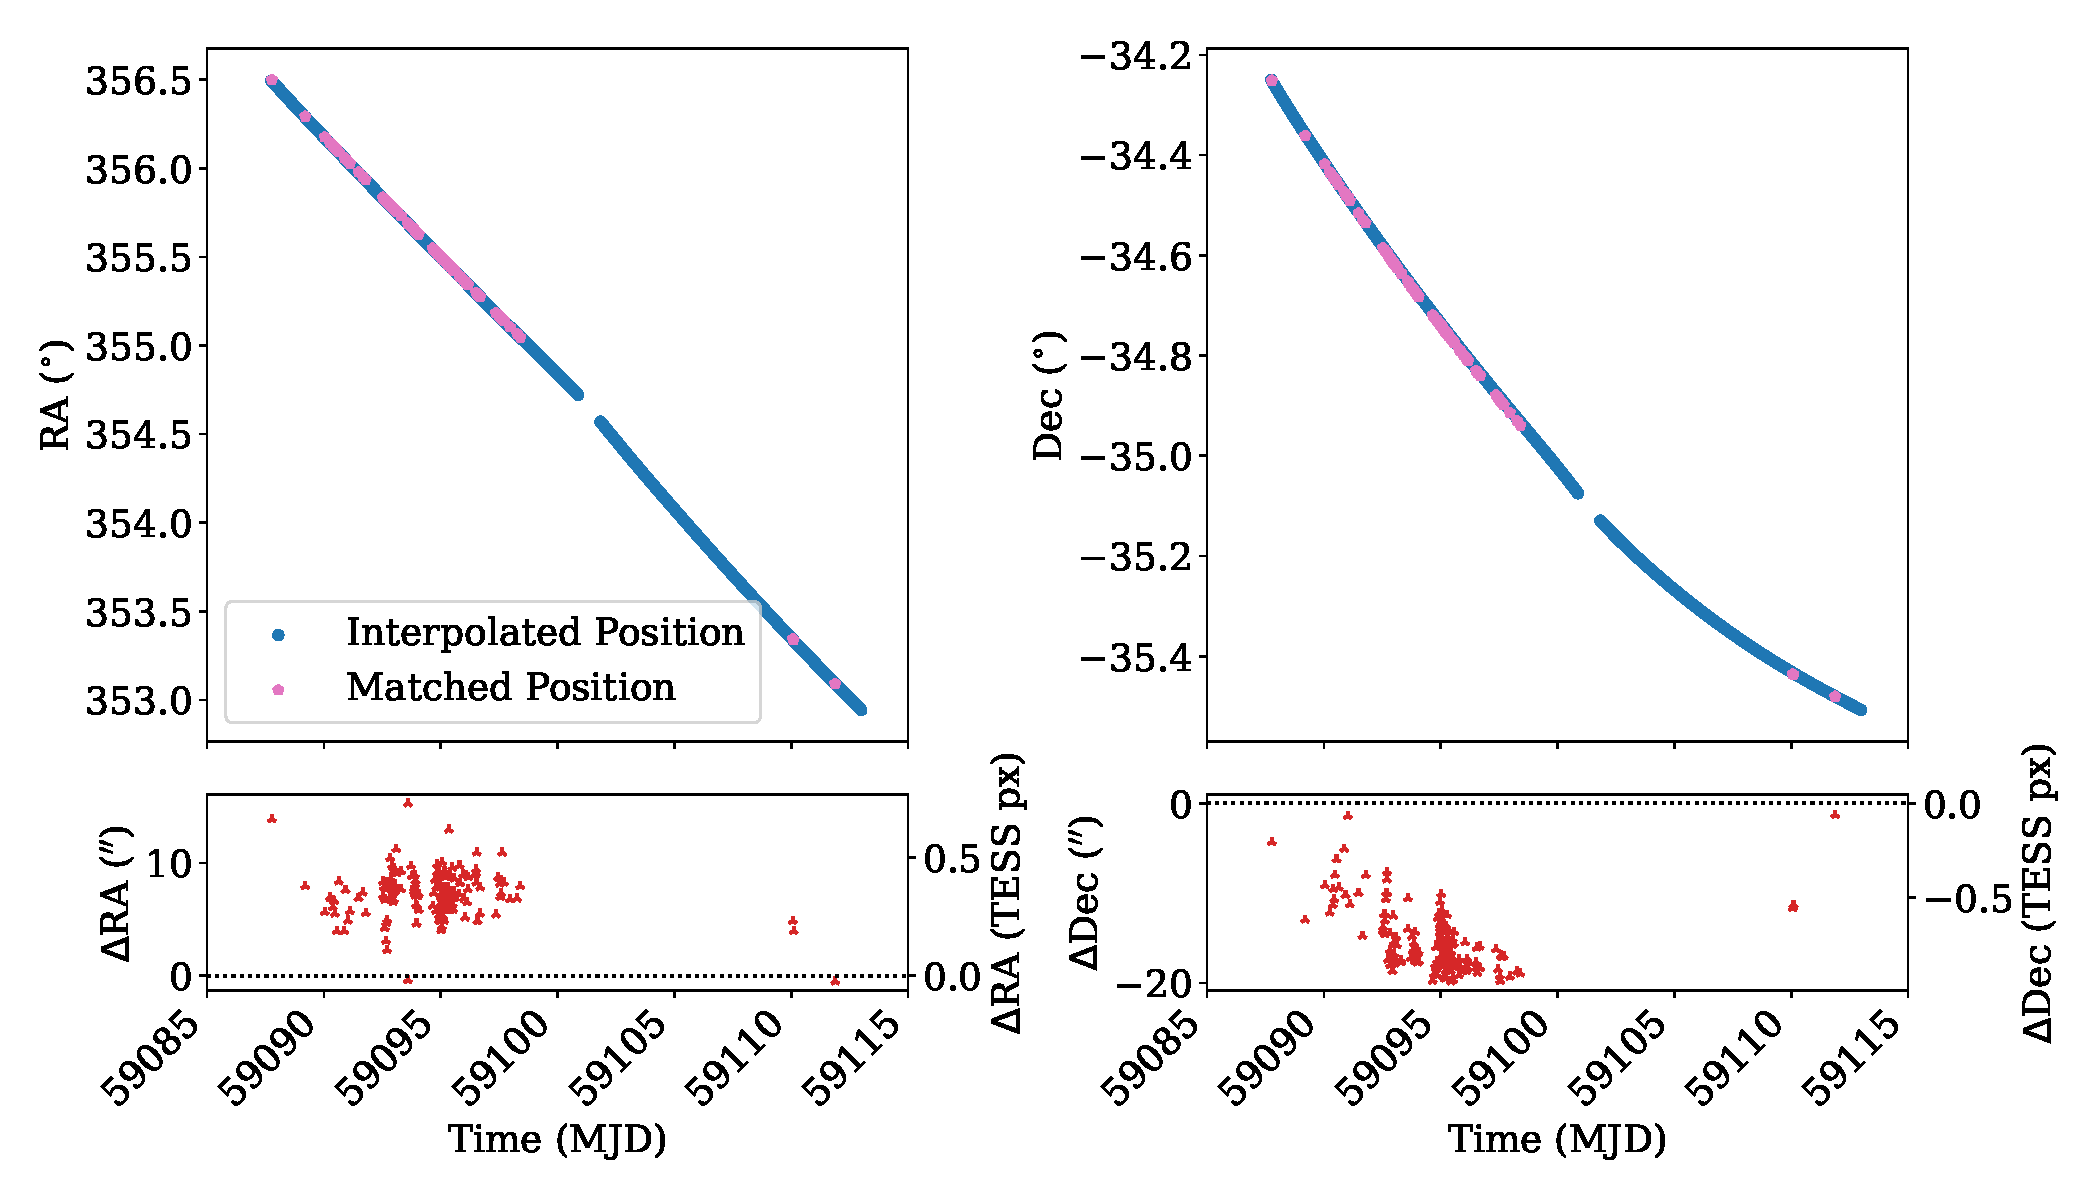
\includegraphics[width =\textwidth]{./Figures/DetectMatchPosUlysses.pdf}
  \caption[Interpolated and Detected Positions]{The RA (right) and Dec (left) of interpolated position (blue dots) or the matches to \texttt{TESSELLATE} detections (pink hexagons) against the time of observation. The lower panels show the residuals of the difference between the positions for points that occur at the same time.}
  \label{Fig:RADecMatch}
\end{figure}

\subsection{Photometry and the Construction of Asteroid Lightcurves}\label{SubSec:Lightcurves}

%light curves; detected VS forced interpolated 
There are two sets of points to take light curves from.
The matches from the detections, which already have a flux calculated, and the interpolated points themselves, which are more numerous but require forcing the photometry.
There were some challenges getting the flux of the interpolated points, even when \texttt{TESSELLATE} has already reduced all the FFIs of interest.

The flux is calculated with \texttt{Photutils} \citep{Bradley2024} aperture photometry with a \qty{1.5}{\px} radius.
This aperture is placed on the centre of mass (COM) position of a $5\times5$ \unit{\px} box around the integer $xy$ coordinate of the asteroid.
The COM was calculate using \texttt{Scipy} and the \texttt{ndimage.center\_of\_mass}.
The integer coordinates are found with the \texttt{SkyCoord} module of \texttt{Astropy}, the world coordinates, in RA and Dec, can be transformed into pixel coordinates, $x$ and $y$, using a world coordinates system (WCS) from TESSELLATE.

The integer coordinates were not used themselves because the asteroids seemed to be leading the object in any given frame of TESS. %?FIG?
This was decreasing the total flux of the asteroid, as the aperture  was hitting mostly background.
This also caused a ``sawtoothing'' effect, where the lightcurve would jump from a minimum to a maximum when the integer coordinate snapped from being a pixel out to back on the asteroid.

I did not take the highest pixel value in a box to make this correction because there could be a rouge star in the field that it detects as the maximum, instead of the asteroid.
The COM technique would still be affected by such contamination, but the magnitude would be less.
The photometry on the COM aperture did fix the sawtoothing, as there is subpixel accuracy in the COM calculation.
There was a far smoother transition from maximum to minimum, as expected from rotating asteroids.
Hereafter, unless otherwise specified, ``flux'' refers to this COM flux measurement of the asteroid.


%TODO data cleaning explaination
A few steps need to be taken to clean these COM lightcurves.
Following \citet{McNeill2023}, any fluxes more than $3\sigma$ from the mean value are sigma-clipped recursivly from the forced photometry lightcurves, until convergence is achieved.
The contamination from background stars the object passes is too great to allow in the lightcurve.
This does introduce gaps into an otherwise regularly sampled lightcurve, but the Lomb-Scargle periodogram is designed to deal with poorly sampled data.
Lightcurves with an average flux $<10$ counts are lost in the random noise floor, so a minimum mean flux limit needs to be applied to ensure quality and reliability of any periods calculated.


The subsections of the FFIs made by \texttt{TESSELLATE} have a small overlap.
If an object moves between these, there will be a few frames where it is found in multiple of these subsections.
This makes the lightcurve have two simultaneous observations of the asteroid, which clearly is not possible.
At the very edge of the subsections, the asteroid can have a COM position that would have the aperture be summing over pixels that are outside the field, and thus the asteroid would have a lower flux value on the edge.
The overlap is great enough that the decrease in flux should only be happening on one of the edges at a time.
So, sorting by flux on a per asteroid basis, then removing the duplicate observation times, keeping only those with the highest flux, will clean the lightcurve.


\begin{figure}
  \centering
  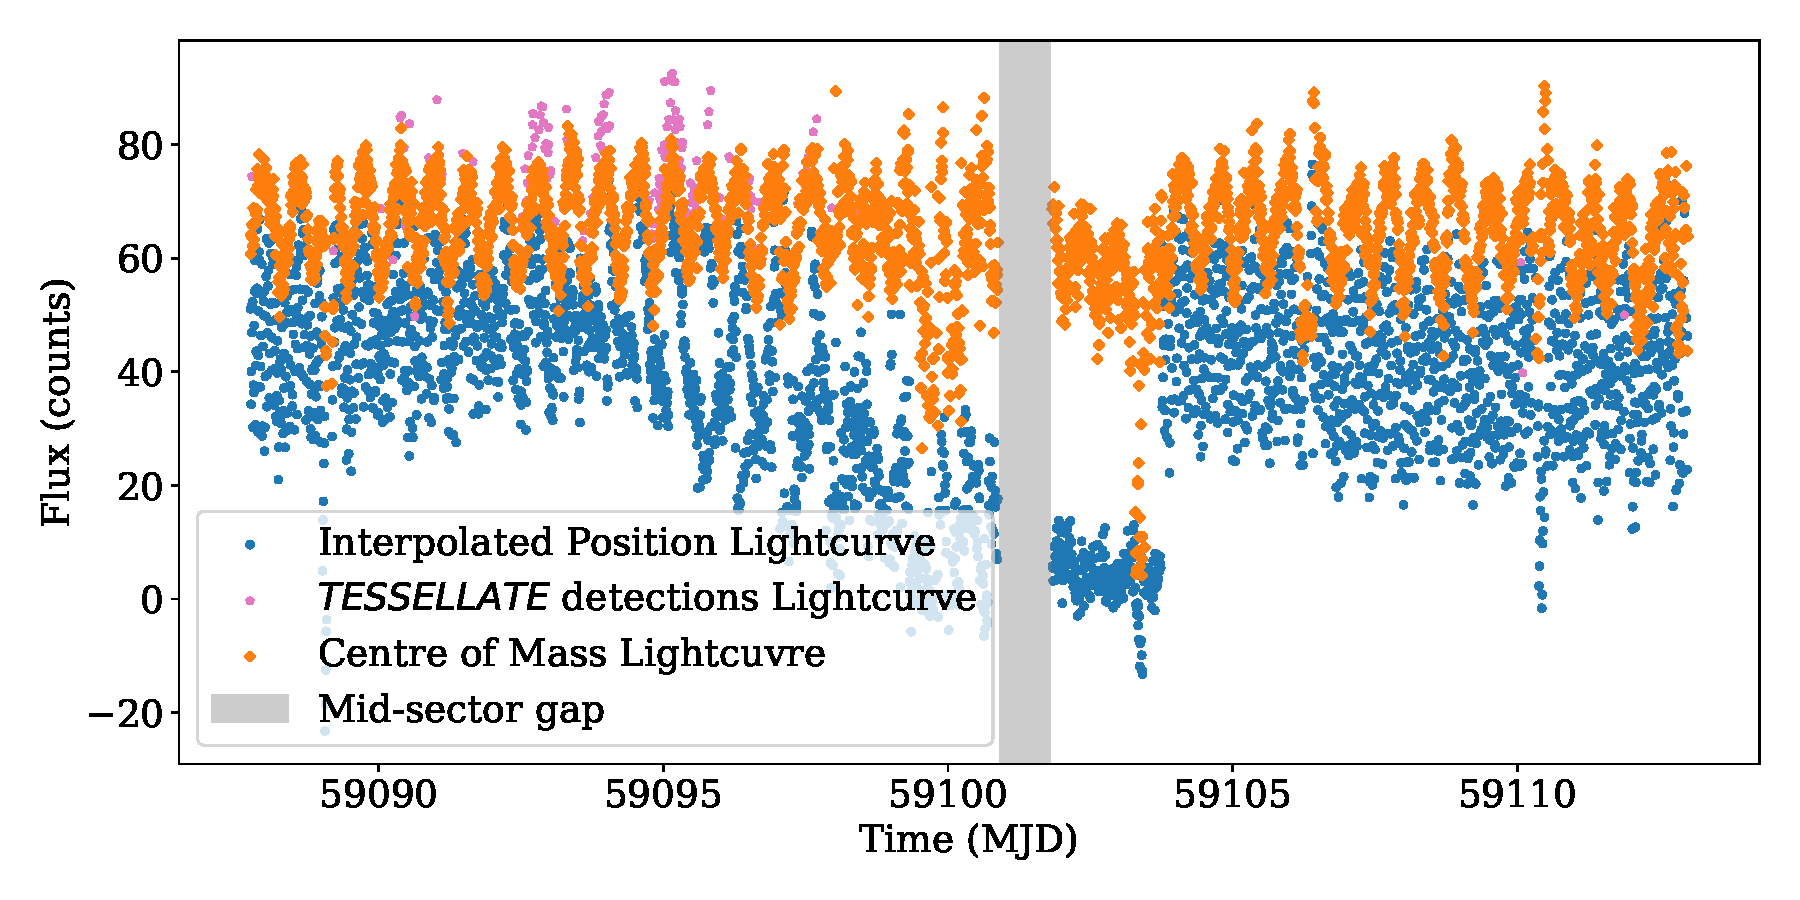
\includegraphics[width =\textwidth]{./Figures/SingleBodyLCUlyssesgapSpan.pdf}
  \caption[Light curves Example]{The light curves of the asteroid (5254) Ulysses throughout its entire journey across sector 29. 
  The flux of the interpolated positions in blue circles,the \texttt{TESSELLATE} flux for any matched points in the pink hexagons, and the COM flux in orange diamonds.
  The mid-sector gap is highlighted by the grey box.}
  \label{Fig:FullSingleLC}
\end{figure}

A comparison between the three light curves is interesting.
\autoref{Fig:FullSingleLC} shows these three light curves for a single body.
The COM flux seems much more stable than the interpolated positions flux, and has a higher average flux count.
This should result in more accurate periodograms as there is less overall variation in the data caused by the misplaced aperture.

The matched points are comparatively sparse for this object, which is not the case for all.
Many have no matches, and some have almost fully matched, as discussed above (\autoref{SubSec:Match}) this will be discussed more later in \autoref{SubSec:Detect}.



\subsection{Calculation of Asteroid Rotation Periods}\label{SubSec:Periods}

%Periods and amplitueds for everything detected
The next part of my analysis involves determining the periods and amplitudes of each asteroid's light curve.
The rotation period and other properties of the lightcurve will be calculated from the forced photometry on the COM positions. the matching is still beneficial to the \texttt{TESSELLATE} pipeline as a whole.
Taking previously unidentified detections and assigning them to an asteroid category, the remaining unknown transients can be more efficiently searched for other interesting astrophysical phenomena.

A widely used technique in determining the periods of astronomical data is the Lomb-Scargle periodogram \citep[\citet{Lomb1976,Scargle1982}, but see][for a review]{VanderPlas2018}.
This method can efficiently take discrete time-series data of which the observations are unevenly spaced and calculate the frequencies present in the sample.
TESS should have rather evenly spaced data, as the FFIs are produced on a set cadence, but sometimes data will be missing.
For example, it may have been sigma clipped due to a spike in brightness that is unphysical for an asteroid, or TESS sees the same asteroid in the same sector on either side of the day long mid-sector break it takes for data transfer.
The periodogram reduces to both a fast Fourier transform or a direct least squares fit in appropriate limits, but outperforms them markedly in unevenly sampled data.

There are a few different implementations of a Lomb-Scargle periodogram available in world of astronomy python packages.
I have used the Lomb-Scargle periodogram as implemented by \texttt{Astropy}\citep[\citet{Astropy2022} but see][for the implementation]{Vanderplas2012,Vanderplas2015}.
The times are converted from MJD into seconds before the periodogram is calculated, so the frequency is calculated in \unit{\hertz}. 
The flux values have their mean subtracted so the change in flux being analysed is about 0 counts.
\texttt{Astropy} has ways of doing this internally, but I opted to do it explicitly.  

\texttt{Astropy} also returns a model, in the form of
\begin{equation}
  \label{Eq:LCModel}
  F(t;f,\vec{\theta}\,) = \theta_0 + \theta_1\cdot\sin{2\pi ft} +\theta_2\cdot\cos{2\pi ft}
\end{equation}
where the flux, $F$, is given in terms of time, $t$, the calculated frequency, $f$, and the model parameter $\vec{\theta} = [\theta_0, \theta_1,\theta_2]$.
These parameters are useful in reconstructing the sinusoid without rerunning the periodogram.
\texttt{Astropy} gives a statistic on how confident it is in the detected frequency is, the false alarm probability.

The method used for the periodogram fits is the new \texttt{nifty-ls} package \citep{Garrison2024} that has can be implemented on its own, or by interfacing with \texttt{Astropy}.
I use the later implementation as the speed-up from the non-uniform fast Fourier transform is helpful.
The large dataset from \texttt{TESSELLATE} requires this calculation efficiency but the \texttt{Astropy} interface is how I was trialling my code on smaller datasets.

The minimum period returned by the periodograms will be set by the Nyquist limit of the data.
For the \qty{10}{\min} FFIs (the cadence analysed here), the Nyquist period is $\qty{20}{\min}=\frac13\unit{\hour}$, a threefold increase in time sensitivity for fast rotating asteroids.
Based on their experimentation with the \qty{30}{\min} cadence FFIs, \citet{McNeill2023} find that periods less than \qty{3}{\hour} be interpreted with caution, due to lack of reliability in recovering injected sources.
Because of the increase in FFI rate, this time will be droped to \qty{1}{\hour} for the minimum reliable period, as the lightcurve sampling on these timescales is equivalent.

A \qty{17}{\day} maximum period for  periodogram analysis follows \citeauthor{McNeill2023}.
A lack of signal in the rotation curve causes the calculated period to default this low frequency limit.
Such cases can be filtered out by keeping only periods less than \qty{90}{\percent} of this maximum.

I originally tried using the \texttt{Lightkurve} \citep{Lightkurve2018} package built for period analysis of TESS (and Kepler) data of variable stars.
There were interesting similarities and differences between the packages.
\texttt{Lightkurve} was easy to use but did not allow for fine-tuning of the periodogram, or give any model of the best-fitting curve it produced.
\texttt{Lightkurve} is based on the \texttt{Astropy} methods, but does not give all the functionality, instead opting to simplify the process.


\begin{figure}[!t]
  \centering
  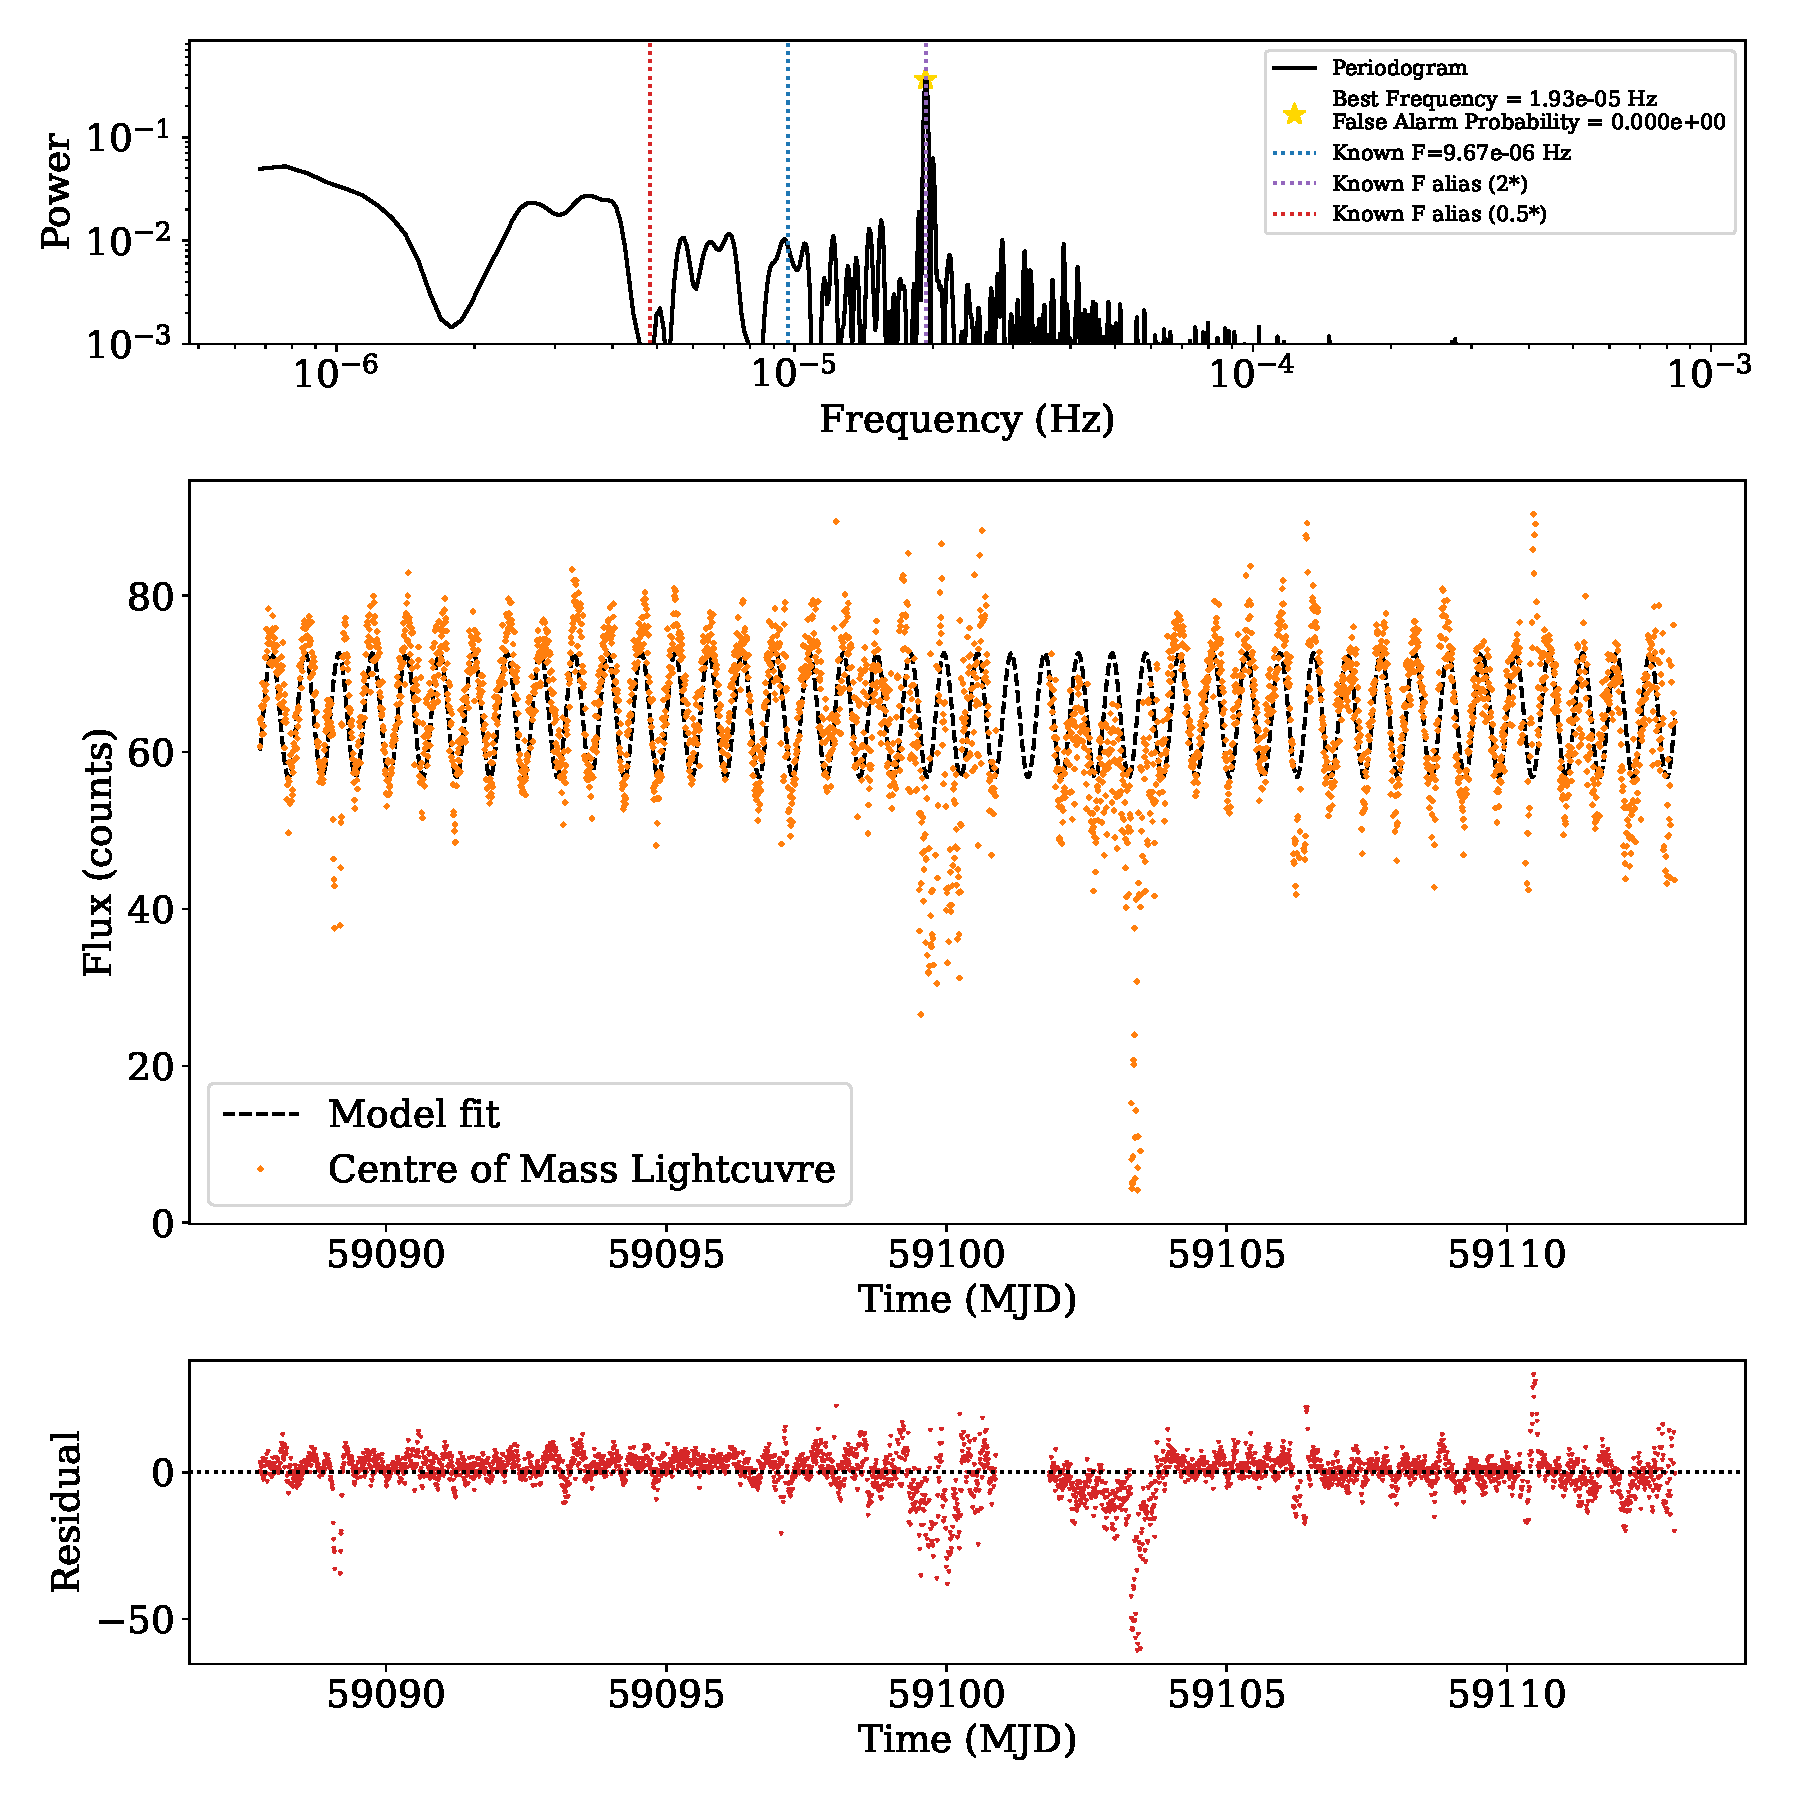
\includegraphics[width=\textwidth]{./Figures/PeriodogramUlyssesResid.pdf}
  \caption[Periodogram example]{\textit{Upper Panel}:The Periodogram of the COM flux of (5254) Ulysses.
    The maximum power of the periodogram is highlighted with the gold star.
    The known frequency, from the LCDB \citep{Warner2009}, is shown in the blue dotted lines, and a factor of 2 alias each way is shown in the purple dotted lines ($2*$) and red dotted lines ($0.5*$).
    \textit{Middle Panel}: The COM flux lightcurve and the returned model (dashed black curve) of the lightcurve from the periodogram analysis.
    The frequency of this model is the same as the gold stared point in the upper panel.
    \textit{Lower Panel}: The residuals of the model fit.
  }
  \label{Fig:PeriodEx}
\end{figure}


An example of such an \texttt{Astropy} Lomb-Scargle periodogram and the corresponding fit to the lightcurve is given \autoref{Fig:PeriodEx}, along with the fit residuals.
The periodogram is limited below at a power of $10^{-3}$ to highlight only the regions with large power. 
The periodogram calculated that this object had a frequency double that listed in the LCDB, as seen with the vertical dotted lines.
This is expected due to the double-peaked nature of most asteroid lightcurves \citep{McNeill2023}.
This asteroid was highlighted as an alias of the known frequency is recovered by this analysis.
To account for this, the detected periods will be doubled for comparison to published works.

The stared peak in \autoref{Fig:PeriodEx} is  the most prominent peak in the periodogram, more that is seems at first glance due to the $\log$ scale.
Not all the asteroids have such well-defined maximums, and the peak power of the periodogram is an important factor in its quality.
A peak power less than 0.1 means there is little to no signal observed and it will be almost indistinguishable from the noise.

The middle panel of \autoref{Fig:PeriodEx} shows the model given in \autoref{Eq:LCModel} fit to the COM flux lightcurve by \texttt{Astropy}.
This looks to be a good fit, with the peaks and troughs lining up.
The amplitude of the sinusoid appears to be slightly lower than the variation of the data, but it is consistent with the scatter.
This model is successfully fit over a break in the lightcurve, and ignores the observations with a lower flux that did not quite get sigma clipped.

The amplitude of the variation is calculated from this model fit.
This is measured in magnitudes, and as such is found from the standard
\begin{equation} \label{Eq:DelMag}
  \Delta m = -2.5 \log_{10}(\frac{F_{min}}{F_{max}})
\end{equation}
with $\Delta m$ being the variation amplitude.
The $F_{min}$ and $F_{max}$ terms in \autoref{Eq:DelMag} and the minimum and maximum flux of the model, respectivly.
These are measured in counts.

The lower panel in \autoref{Fig:PeriodEx} shows the residuals of the model subtracted from the data.
For the majority of the observations, the residuals are close to the 0 line, indicating a high quality fit.
There are places where there is a significant deviation from 0, corresponding to places in the lightcurve that look out of place to the eye. 
These large residuals could be removed by decreasing the tollerance on the sigma clipping, but that could cut true signal in lightcurves with a large variation amplitude. 


\subsection{Periodogram Quality Checks}\label{SubSec:QualCheck}

For accurate statistics, reliable data is needed.
So there must be checks on the quality of the values calculated.
Some of these have been discussed already, but for completeness I list again here.
A lightcurve must have a mean flux of at least 10 counts to be reliable.
For an accurate periodogram, it is required that the lightcurve also contain more than 200 observations, which is very easy for TESS and its \qty{10}{\minute} cadence, as the asteroid only has to be in the sector for \qty{33.3}{\hour}.
The periodogram itself must have a peak power of at least 0.1 to be distinguished from the noise
The calculated period must be $\qty{1}{\hour}\leq P \leq \qty{367.2}{\hour}$, where the upper bound is \qty{90}{\percent} of the \qty{17}{\day} window suggested by \cite{McNeill2023}.


\section{Results}\label{Sec:Res}

Here I present the results for TESS sector 29.
Similar analysis can be preformed, and the same figures made, for any of the sectors.
The computation time was a limiting factor in getting more sectors processed.
There were 5664 objects detected in the sector with $V\leq \qty{20}{\mag}$, of which 374 passed all the quality checks imposed on their lightcurve and periodogram.  


\subsection{Quality Check Verification}\label{SubSec:QualCheckVer}

\begin{figure}[t]
  \centering
  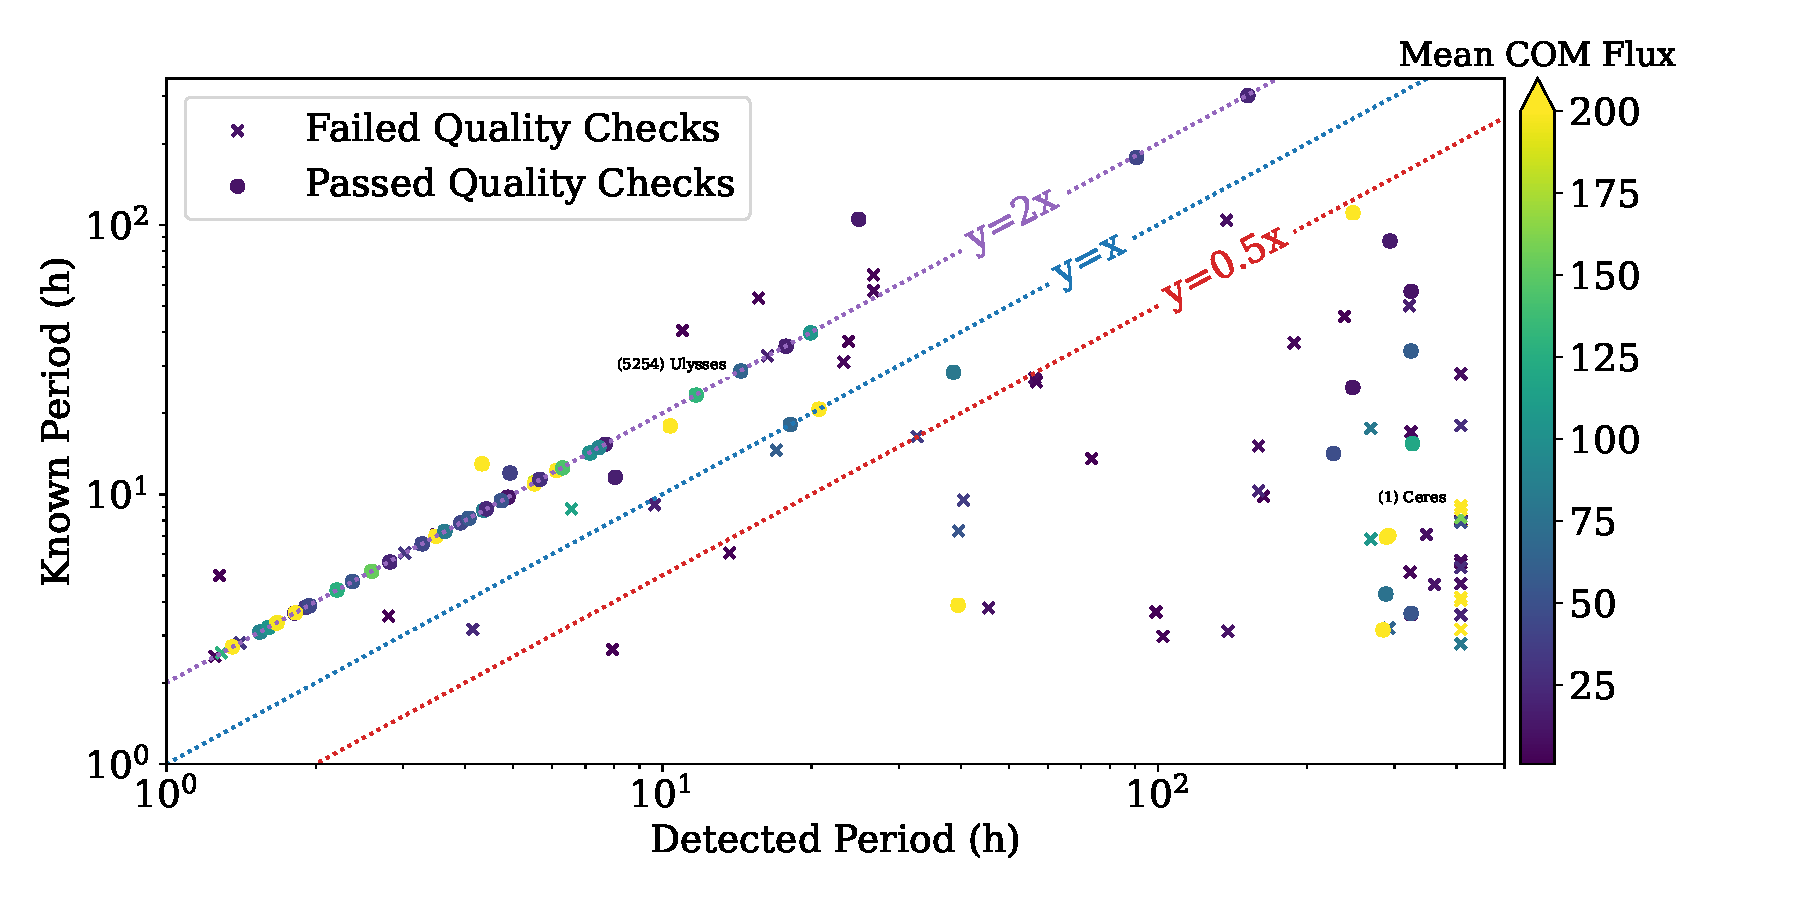
\includegraphics[width=\textwidth]{./Figures/LCBDcompFinal.pdf}
  \caption[LCDB known period against detected period]{A comparison of the detected periods of the objects in the sector to their known periods in the LCDB \citep{Warner2009}, coloured by the mean flux of the object.
  Crosses failed the quality checks, while circles passed them.
  Names of asteroids are referring to the data point to the right of the text.
    Dotted lines of a constant relationship are plotted, coloured the same as \autoref{Fig:PeriodEx}.
  }
  \label{Fig:LCDBcomp}
\end{figure}

While some quality checks were chosen to agree with the past work of others, some were chosen to make sure the derived periods were in agreement with the known ones from the LCDB.
A comparison between objects in both the sector and the LCDB is seen in \autoref{Fig:LCDBcomp}.
Of the 121 objects in both samples, 59 of them passed all the checks.
These are included in the total 374 asteroids that pass  all the quality checks in sector 29.
This means over \qty{80}{\percent} of the asteroids that pass all the checks do not have known periods.

\autoref{Fig:LCDBcomp} is coloured by the flux of the asteroid to give an idea of what quality check the object failed. 
If a cross is bright yellow, the periodogram checks would have been responsible, as the average flux is well above the necessary 10 counts.
The one bright asteroid that failed the checks in the top left is right on the boundary of the \qty{1}{\hour} lower limit, indicating that this bound may be slightly too lenient.
The vertical line of points on the right-hand side of \autoref{Fig:LCDBcomp} is on that maximum of the window of searched periods at $\qty{408}{\hour}$, and demonstrates why the \qty{90}{\percent} upper bound is necessary.
Many asteroids, across an order of magnitude of known periods and across the range of mean fluxes, have detected periods at the edge of the window, showing that the periodogram will return this value when no signal is present.

The largest asteroid, (1) Ceres, is highlighted in \autoref{Fig:LCDBcomp}. 
It is not recovered, as it is almost too bright for TESS, and the flux bleeds into too many pixels for a rotation period to be accurately obtained from the \qty{1.5}{\px} aperture used.
An exception to the methods is not made here, no reanalysis is attempted.
This object is the main reason for the arrow on the colour bar indicating higher mean flux values without a change in colour.
(1) Ceres has a mean flux is over 100000 counts which, if included, completely washes out the gradient.
200 counts was chosen as a replacement value because of the range of detail that can be identified. 


The brightness of those asteroids that passed the checks is also useful to see.
If a circle is dark blue, it may only just be above the minimum requirements for average flux.
The bright circles in the lower right of \autoref{Fig:LCDBcomp} are cause for concern, as these are bright asteroids that are passing the checks with an incorrect period. 
A range of brightness pass the checks, indicating sensitivity to a wide range of distances and sizes.
These are the two competing effects that determine the average flux of an object, those that are further away need to be larger to reflect the same amount of light to the detector.

The $y=2x$ line of \autoref{Fig:LCDBcomp} is of interest here, the known periods being twice the detected period.
This line corresponds to the calculated frequency being an alias of double the known frequency, as frequency and period are inverses of each other.
This is expected \citep{McNeill2023}, this line is what the periodogram should return due to double-peaked lightcurves.
As seen in \autoref{Fig:PeriodEx}, (5254) Ulysses falls on this line, highlighted by text in \autoref{Fig:LCDBcomp}.
Most of the asteroids the pass the cut line along or near this key relation.
Few asteroids on the line fail the checks, which is also reassuring that the checks do what they are supposed to and filter out incorrect periods.

There are about a dozen asteroids that pass the checks with large detected periods when compared to their known period. 
These points in the lower right of \autoref{Fig:LCDBcomp} imply the checks are not perfect.
Some experimentation was done on the limiting values, and the ones presented here achieved the highest recovery of accurate asteroid periods, while minimising the number that were incorrectly recovered.

The idea of doubling the detected period of all the asteroids and calling that number the rotation period has had some doubt cast on it, as there are a couple of points recovered nicely on the $y=x$ line, indicating that the true period is found.
Either the LCDB has not accounted for the alias, which is unlikely as I only took the periods with high quality codes as they suggest \citep{Warner2009}, or the rotation signal sometimes returns the true period.
The latter implies the lightcurve is not double-peaked, as is normally expected.
On the whole, there are enough periods that pass the checks with incorrect periods that these extra erroneous periods will not significantly change the fraction of reliable detections.


\subsection{Asteroid Properties}\label{SubSec:AstPropRes} %TODO fix name

A plot of the semi-major axis against the other proper elements, eccentricity and inclination, is shown in \autoref{Fig:AEI}.
Looking at the data as a whole, all objects in the field of the instrument during the sector, with $V \leq \qty{20}{\mag}$, are plotted.
The exception being centaurs, which have an $a$ too larger for the detail in the distribution of the majority of the objects to be seen, and comets, which have an undefined $a$.
The 374 objects that passed all the quality checks have a similar distribution of orbital parameters to the total sample of 5664 small bodies in the sector. 
This shows just how beneficial TESS is, and why its full sky coverage is so important to solarsystem science. 

The distinction between the resonances in the main belt can be seen.
There are vertical strips separating the middle belt from the inner and outer belt.
The Jupiter Trojans are well-defined, at just past \qty{5}{\au}, with a small range of eccentricity but a large spread in the inclination.
A some Mars crossers and near earth asteroids (NEAs) at progressively smaller $a$ and a few more objects that are scattered with high $e$ and/or $i$ complete the distribution.
Many objects have failed the quality checks on their lightcurve and periodogram, but the ones that pass have a similar distribution in orbital parameters to the sample as a whole.

\begin{figure}
  \centering
  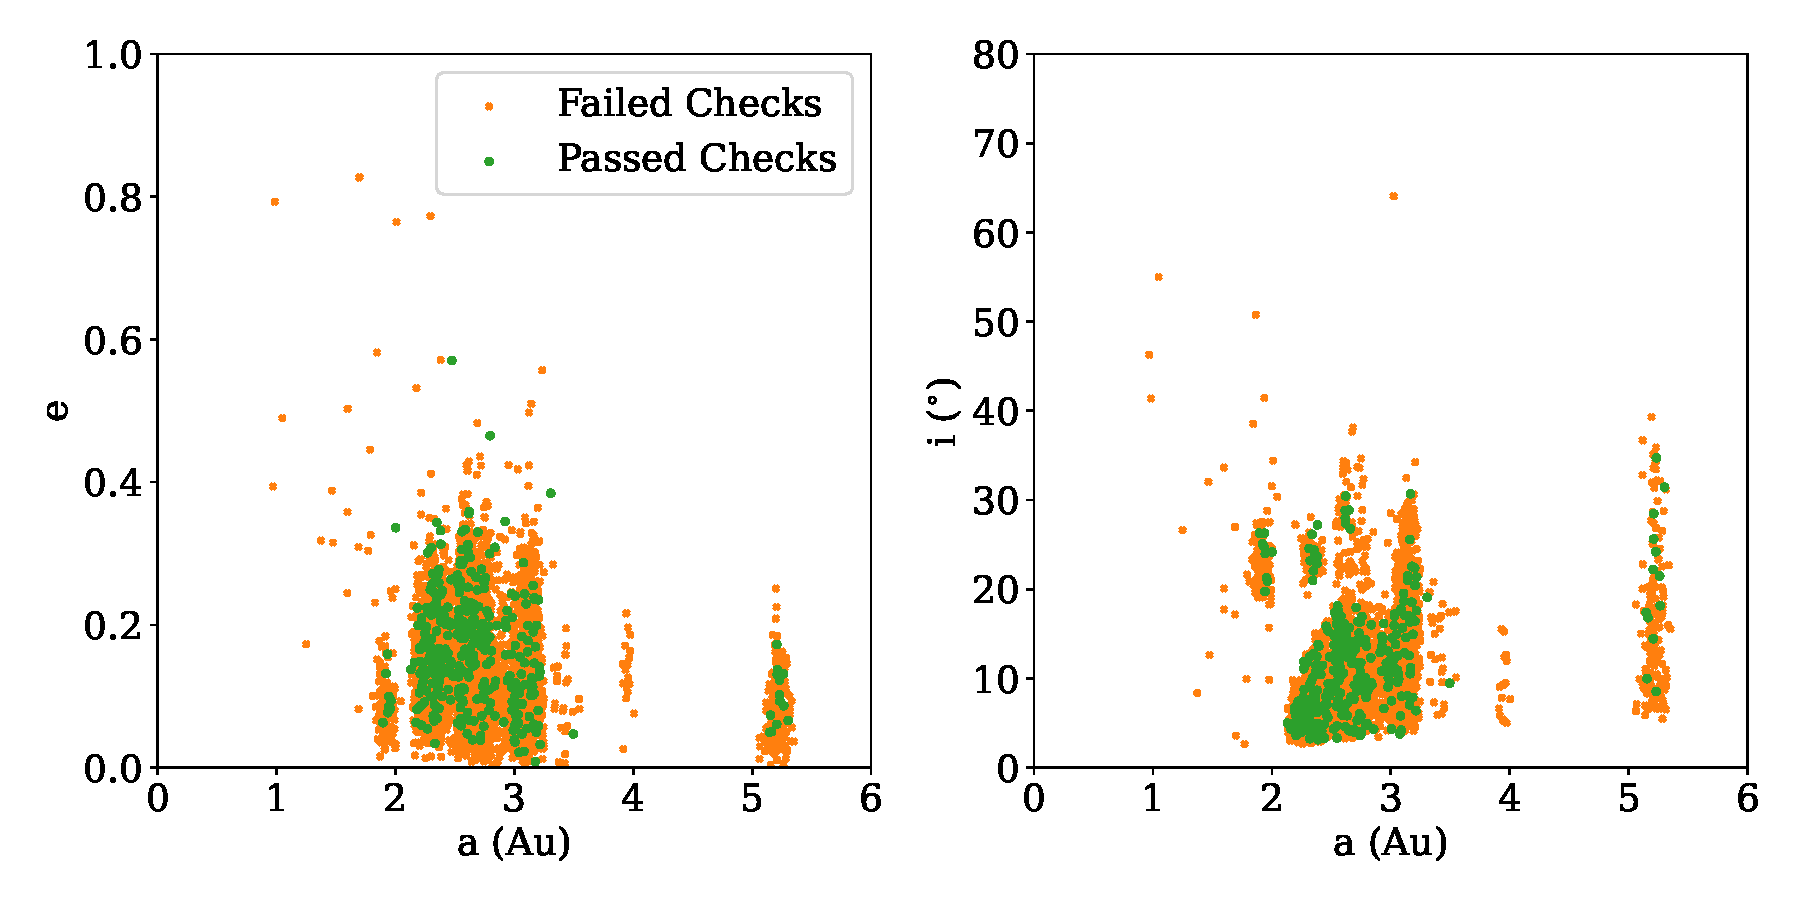
\includegraphics[width=\textwidth]{./Figures/AEIplotqualCut.pdf}
  \caption[aei distribution]{
    The $a$ against both $e$ and $i$ of the objects that \texttt{SkyBoT} found in Sector 29 with $V <\qty{20}{\mag}$.
    The orange crosses are those objects that did not pass the quality checks on the lightcurve and periodogram, while the green is those that did.
    The values of these proper elements were queried from \texttt{JPL Horizons} on 30/09/24.
  }
  \label{Fig:AEI}
\end{figure}

The number of asteroids belonging to each class of objects is highlighted in \autoref{Fig:NumPerClass}.
As expected from the orbital elements in \autoref{Fig:AEI}, the majority of the minor planets fall in the three regions of the main belt.
There are some objects that are not asteroids, 20 comets were in the field and 1 centaur.
While they have a V mag less than 20, these objects are often not bright enough to have lightcurves with high enough mean fluxes to be detected well by TESS.
As seen by the green bars in \autoref{Fig:NumPerClass}, around \qty{5}{\percent} of any class have lightcurves and periodograms that pass the quality checks, and this is relatively class independent.
The highest fraction is the detection of 1 object in the Amor family of NEAs.
However, with only 9 total objects in the dataset, the sample is too small to make claims on the detectability of this class as a whole.

\begin{figure}
  \centering
  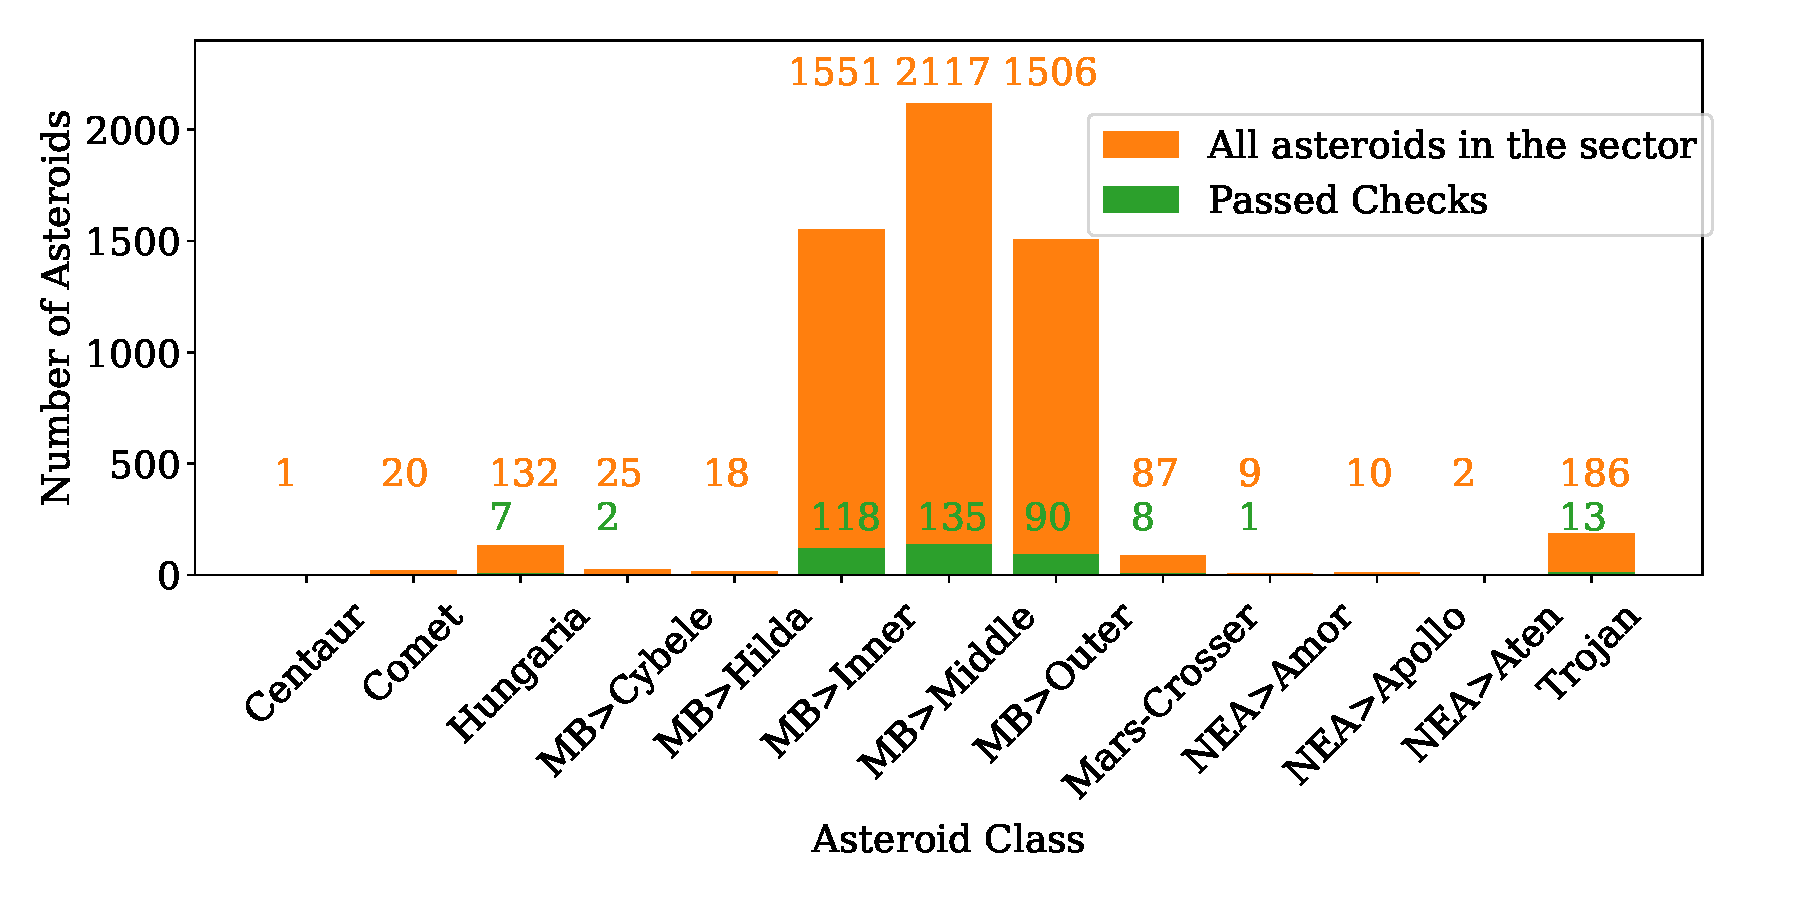
\includegraphics[width=\textwidth]{./Figures/classesBarqualCut.pdf}
  \caption[Class distribution]{A bar chart distribution of the total number of objects per class that \texttt{SkyBoT} found in the Sector (orange) and the same distribution of those that passed all the quality checks (green).
    The numbers above each class (coloured the same) correspond to the height of the bar, as some classes have too few objects to be seen.
    As with \autoref{Fig:AEI}, this is for all objects brighter than \nth{20}\unit{\mag}.
    For the class labels, MB is ``main belt'' and ``NEA'' is near earth asteroid.}
  \label{Fig:NumPerClass}
\end{figure}

\subsection{Asteroid Detectability in TESS} \label{SubSec:Detect}

\begin{figure}
  \centering
  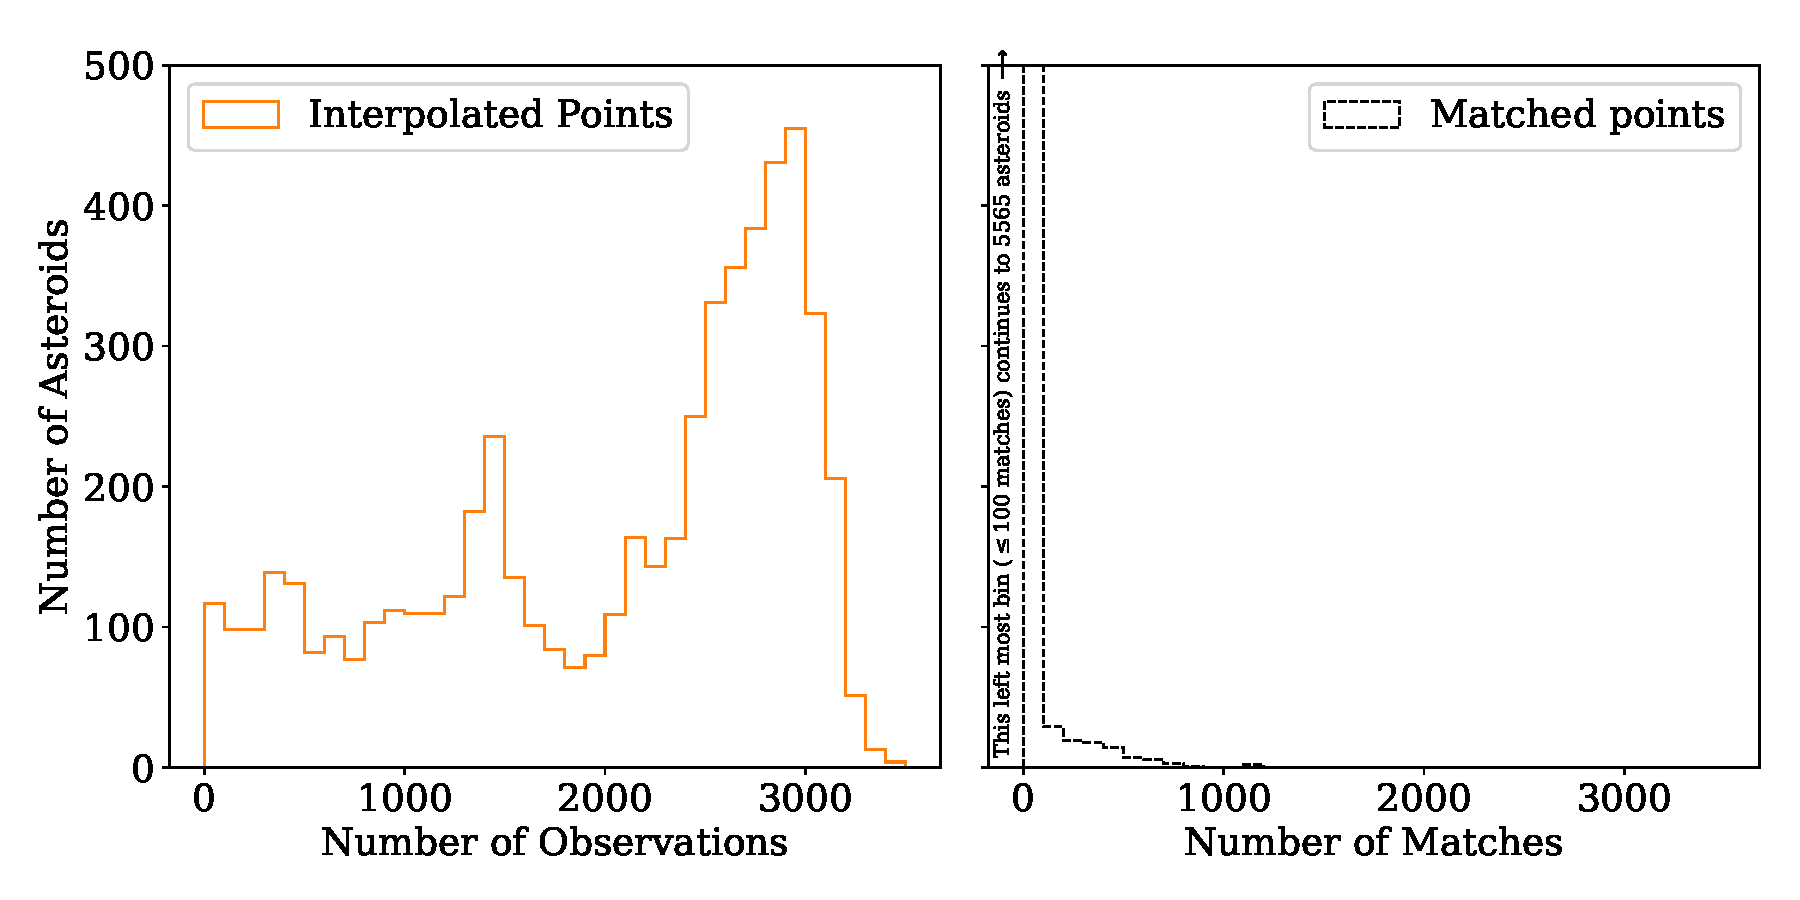
\includegraphics[width=\textwidth]{./Figures/pointsMatchesNumberHistdoubleChangedbound.pdf}
  \caption[Number of observations or matches]{\textit{Left}: A histogram of the number of observations in the lightcurve of each asteroid (orange solid line) in 100 observation bins. \textit{Right}: The number of matches each asteroid gets in the \texttt{TESSELLATE} detections (black dashed).
  }
  \label{Fig:MatchInterpHists}
\end{figure}

The number of forced photometry observations in a lightcurve is more evenly distributed than the number of matches, as shown in \autoref{Fig:MatchInterpHists}.
The quality cut of 200 observations in a lightcurve only cuts out $\sim 200$ asteroids.
Most asteroids are well sampled, with the mode of the distribution in the 2900 to 3000 observation bin, which means the asteroids are in a large fraction of the about 3500 frames in a sector.

The matches have a very different distribution to the observations.
While both plots are limited to 500 asteroids on the y-axis, the matches' histogram in the right plot far exceeds this in the first bin, $\leq$ 100 matches, as indicated by the text and arrow.
Yet the y-limit is too large for detail to be seen in any higher bin of this plot.
There are only a total of 101 asteroids, out of the 5664 in the sector, that are matched more than 100 times to \texttt{TESSELLATE} detections.
So using the matches as lightcurves for periodogram analysis would mean most fail the minimum observations check, which limits the sample before any periods are calculated.

\begin{figure}
  \centering
  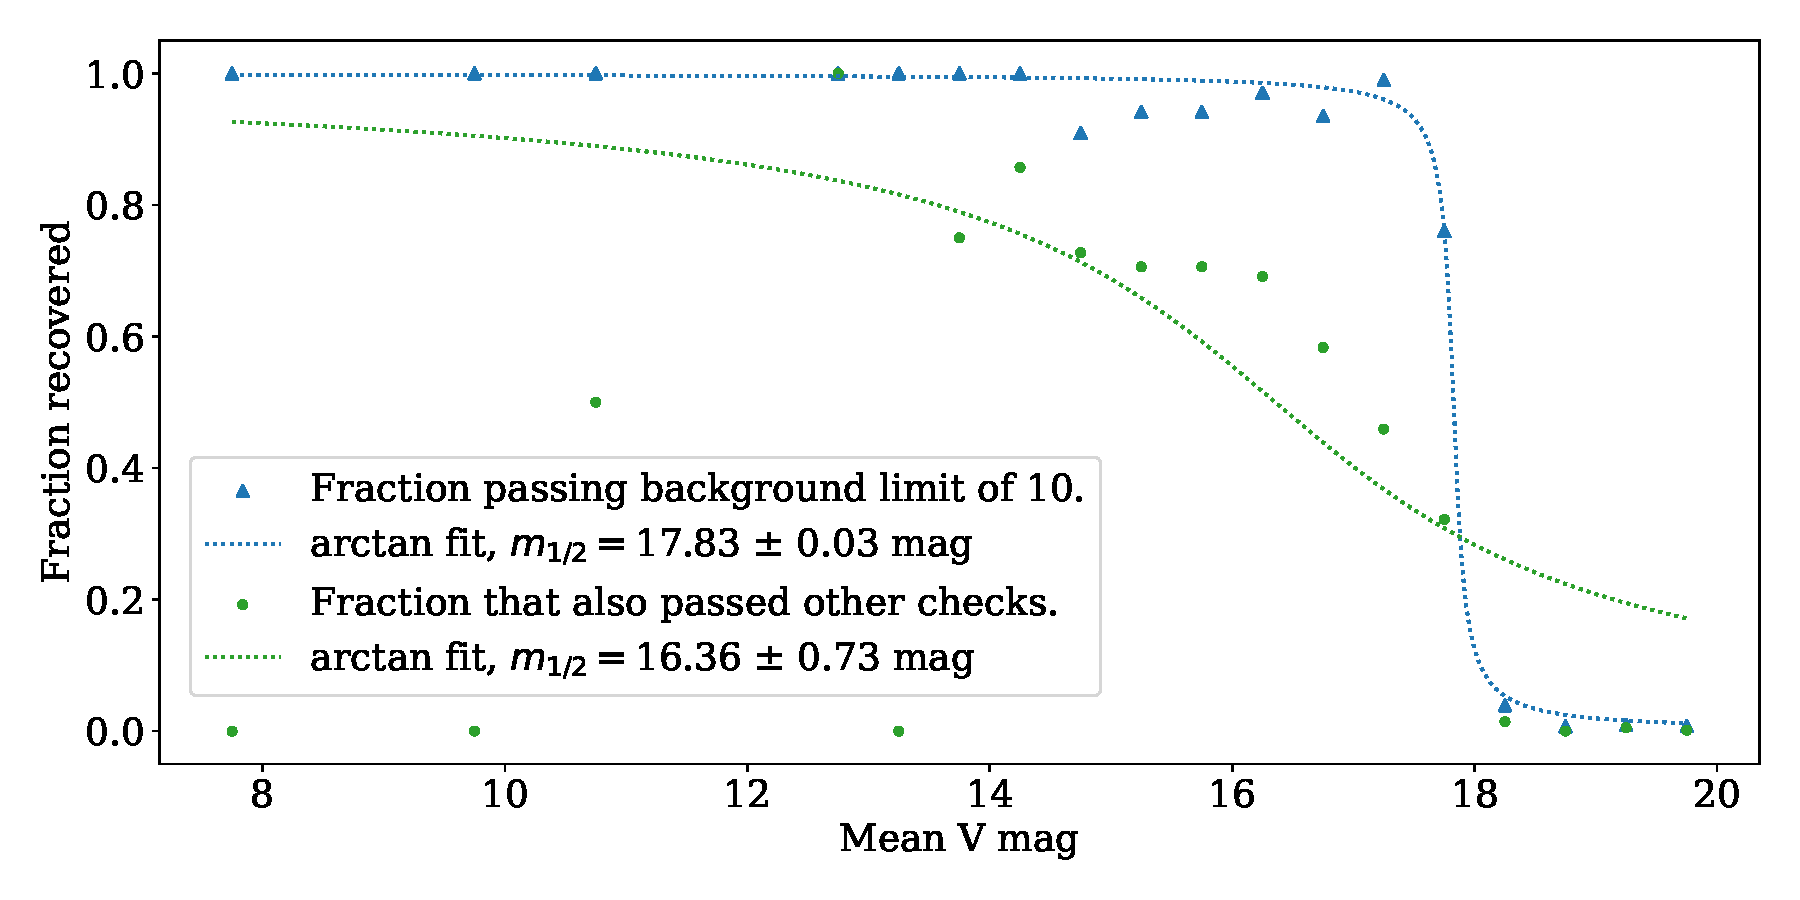
\includegraphics[width=\textwidth]{./Figures/recoverdHistBkgLimof10AtanBothLegendFixed.pdf}
  \caption[Visual Magnitude Recovery]{The recovery fraction against the known visual magnitude of each object in \qty{0.25}{\mag} bins.
  Coloured by whether the object exceeds only the mean flux requirement of the quality checks (blue triangles) or passes all the quality checks on the lightcurve and periodogram (green circles).
    A fit of an $\arctan$ function is provided in dotted lines of the same colour.
  }
  \label{Fig:RecovPassorFail}
\end{figure}

It is clear for \autoref{Fig:RecovPassorFail} that the mean flux check prohibits most of the asteroids dimmer than \nth{18} \unit{\mag}  from being detected. 
The other checks cut down in the middle of the brightness range of objects rather evenly.
The brightest bins, which only have a handful of asteroids in them are not reliable data points, as the values they can take on are too discrete.
(1) Ceres has $V<\qty{8}{\mag}$ and is not recovered, as discussed in \autoref{SubSec:QualCheckVer}, and is the only object in this magnitude bin, so a 0 recovery fraction is returned.  


The fits of to the fraction recovered in \autoref{Fig:RecovPassorFail} take the form
\begin{equation} \label{Eq:Atan}
  y= 0.5 -\frac{1}{\pi} \arctan(\alpha \cdot (m-m_{1/2}))
\end{equation}
where $y$ is the recovered fraction, $\alpha$ is how the steep the transition from 1 down to 0 is,  $m$ the magnitude and $m_{1/2}$ is the shift along the magnitude axis.
The constant of 0.5 in \autoref{Eq:Atan} raises the point of inflection to be at $\frac 1/2$, and the $\frac{-1}{\pi}$ makes the function take the expected maximum at bright magnitudes at \qty{100}{\percent} recovered, down to no dim asteroids being detected.
The $m_{1/2}$ parameter dictates the limiting magnitude, as dimmer than this value less than half of the asteroids are recovered.
The fit is preformed on all bins (of \qty{0.5}{\mag}) dimmer than the first bin with more than one asteroid in it, to stop the discrete values from extremely bright asteroids from having too much influence.

There is a significant change in $m_{1/2}$ between the recovery curves in \autoref{Fig:RecovPassorFail}.
When only the minimum average flux of 10 counts requirement is applied, the limiting magnitude is \qty{17.78(0.01)}{\mag}.
When all the quality checks are imposed, this gets over a \unit{\mag} brighter, to \qty{16.46(0.37)}{\mag}.
It is expected that a higher threshold for quality will make the limiting magnitude brighter.
The $m_{1/2}$ for the full suite of quality checks is rather  uncertain because of the scatter in the recovery fraction at brighter magnitudes, and the shallower decrease in efficiency.


\subsection{Rotation Period Analysis Results}\label{SubSec:PerRes}

For the 374 asteroids that pass the quality checks, relable rotation periods are obtained.
\autoref{Fig:PerDistr} shows the distribution of these rotation rates. 
The period plotted is double the detected period, to account for the double peaked nature of most lightcurves.
The mode of the distribution is a period less that \qty{1}{\day}, by a factor of 10 over periods in the \qtyrange{1}{2}{\day} bin, the \nth{2} most populated.  


\begin{figure}
  \centering
  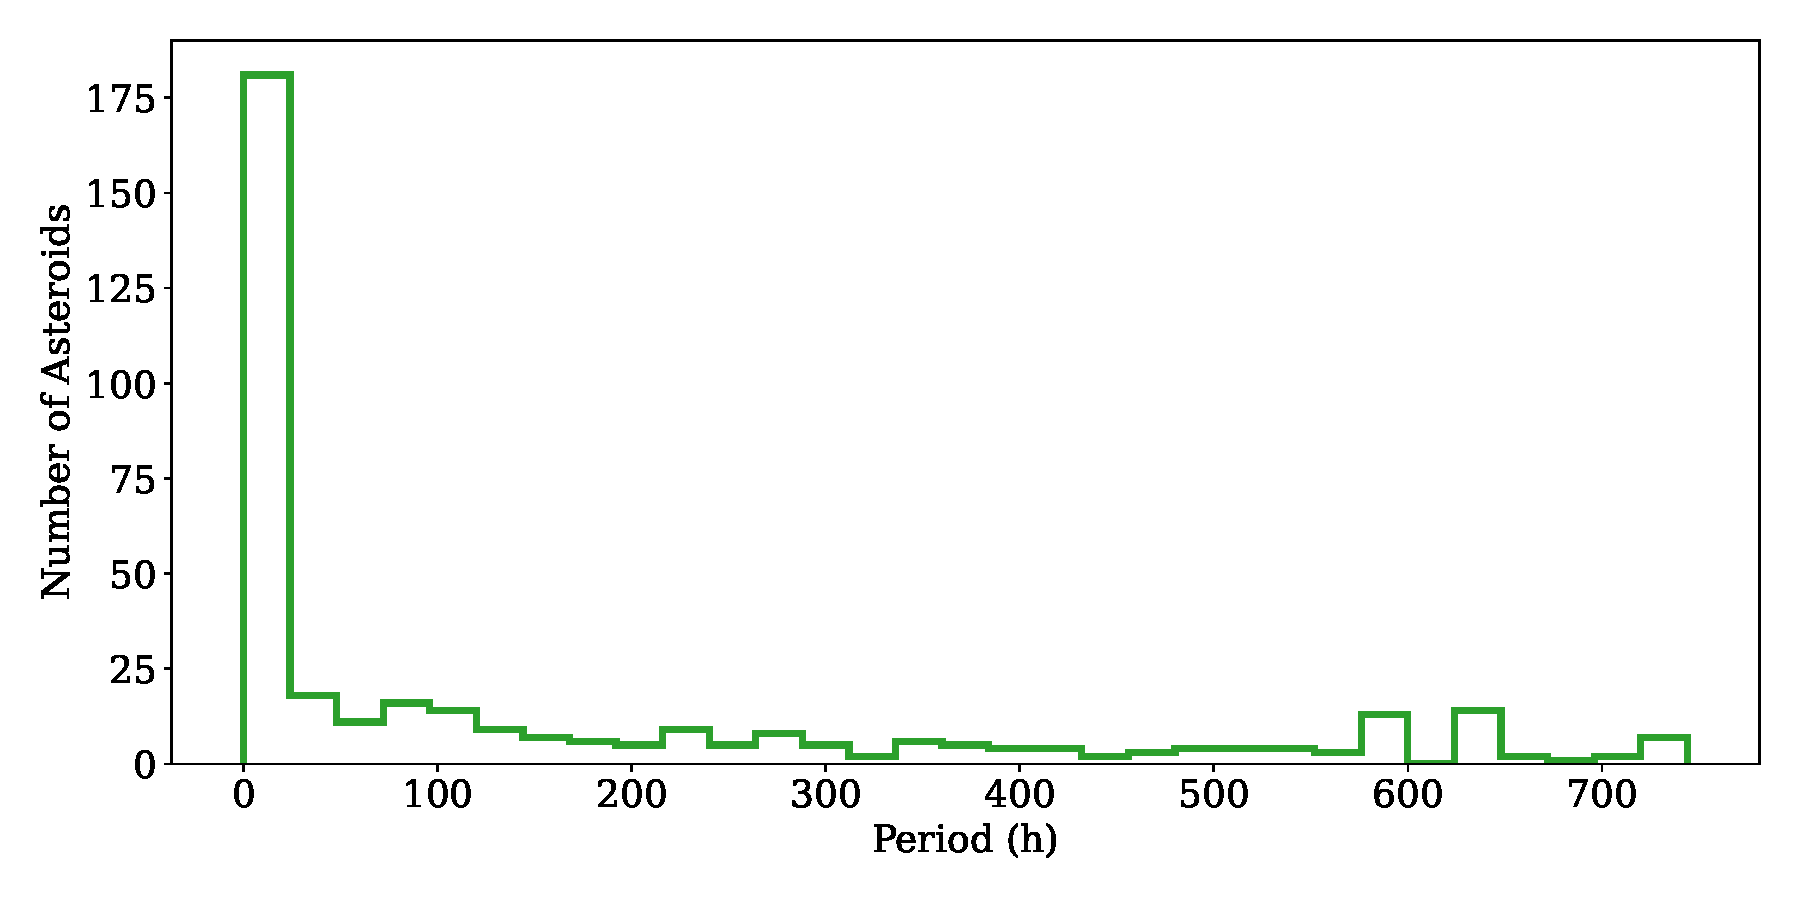
\includegraphics[width=\textwidth]{./Figures/perDistr.pdf}
  \caption[Period Distribution]{The distribution of rotation periods in \qty{24}{\hour} (\qty{1}{\day}) bins for all the asteroids that passed the quality checks.}
  \label{Fig:PerDistr}
\end{figure}

The distribution of the amplitude of the lightcurves is given in \autoref{Fig:ampDistr}.
The peak of the distrabution at $\frac13$ \unit{\mag} and is right skewed.
The high $\Delta m$ values are from lightcurves of dubious quality. 
Manually checking the analysis, it is clear that these points above $\Delta m =2$ have all been affected by background contamination, and have untrustworth photometry.
Some examples are given in the appendix for asteroids with known periods.

It is unclear how to avoid such contamination.
For some, analysis of the residuals could show a pattern that leads to a period and possible fit of a model, but this is not the case for all of them.
For only one sector worth of data, it was managable for me to preform a manual check on these few outliers
But this will not be the case for all the whole dataset \texttt{TESSELLATE} will analyse. 


\begin{figure}
  \centering
  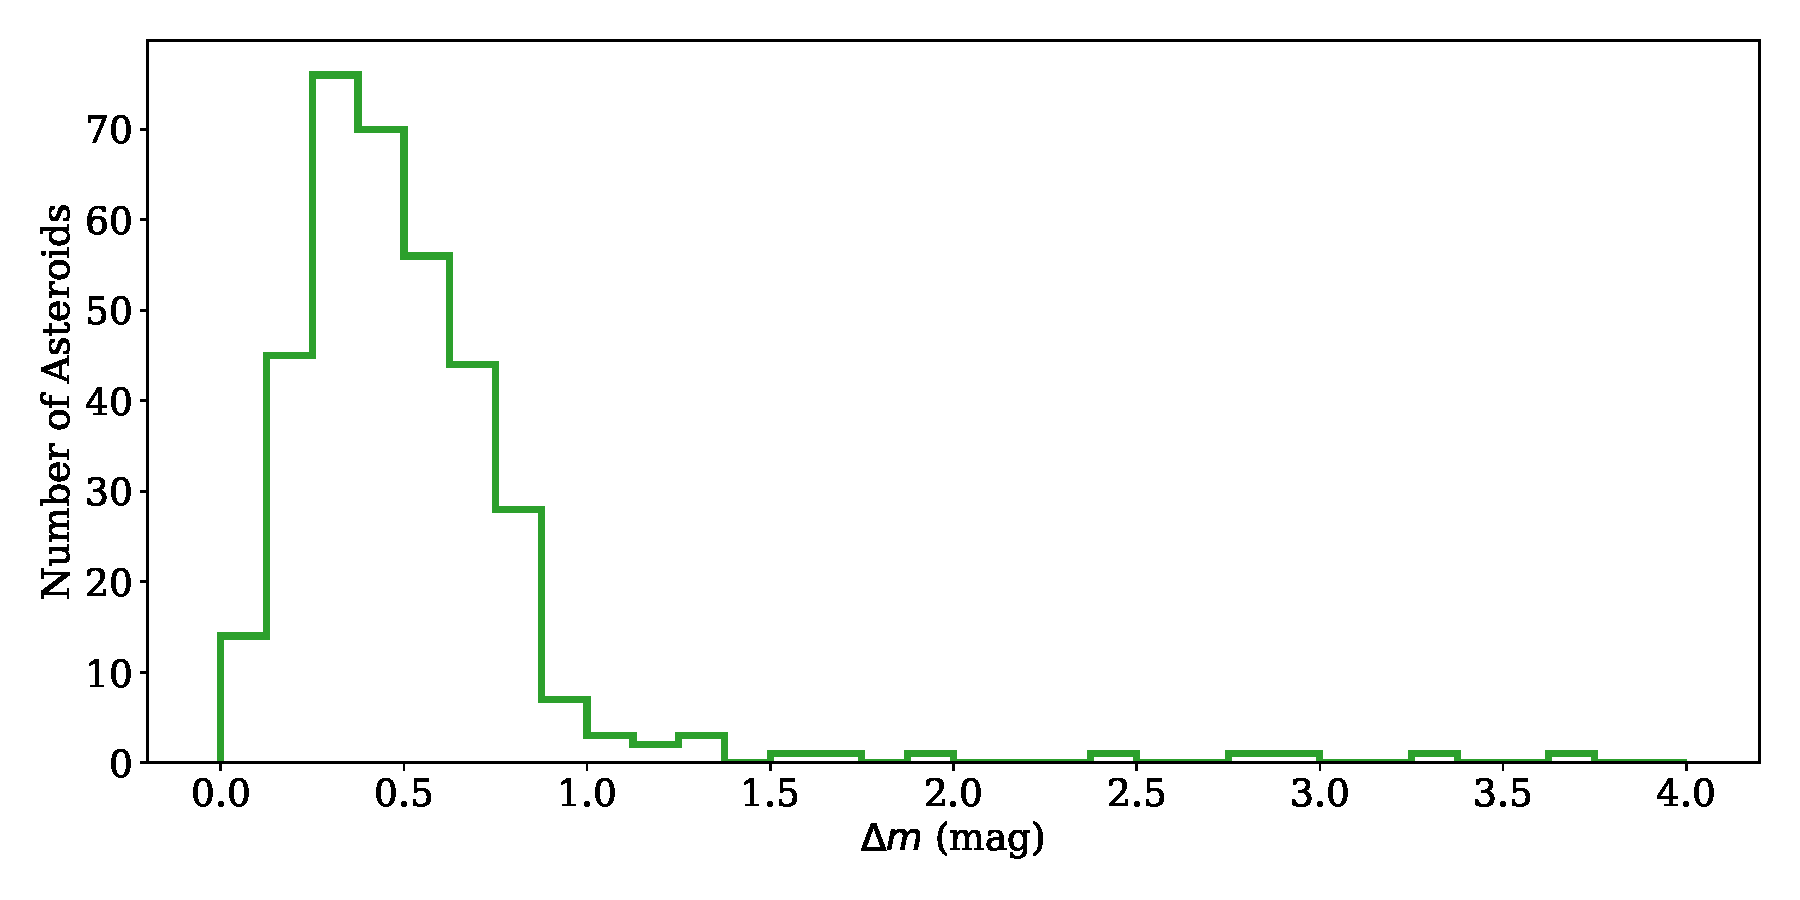
\includegraphics[width=\textwidth]{./Figures/delMagDistr.pdf}
  \caption[Amplitude Variation Distribution]{The distribution of amplitude variation for all the asteroids that passed the quality checks. 
  The data are binned in steps of $\frac{1}{8}$ \unit{\mag}.
  }
  \label{Fig:ampDistr}
\end{figure}

\begin{figure}
  \centering
  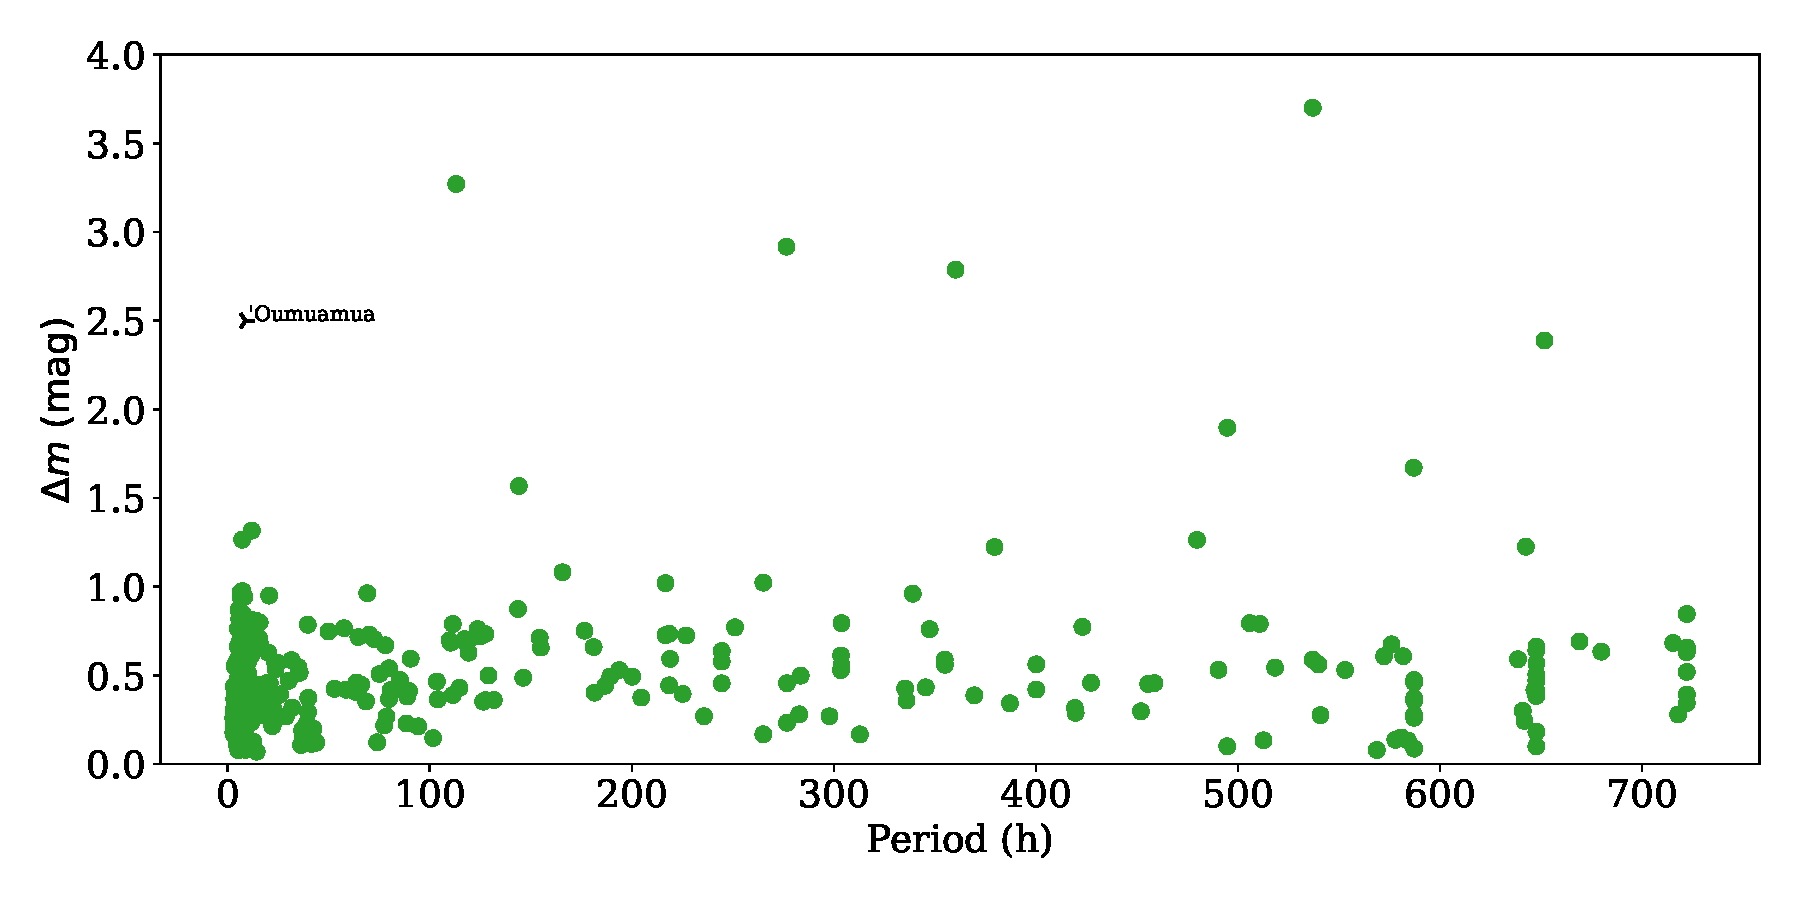
\includegraphics[width = \textwidth]{./Figures/QualPervsAmp1I.pdf}
  \caption[Amplitude of Variation against Rotation Period]{The amplitude of variation in the model from the period analysis against the calculated rotation period.
    This is for all 374 %!CHECK
    objects that pass the quality checks.
  }
  \label{Fig:perVSamp}
\end{figure}


\section{Discussion}\label{Sec:Disc}

\subsection{Comparison to other work }%\citet{McNeill2023}}

%TODO redo fig 1

\begin{figure}
  \centering
  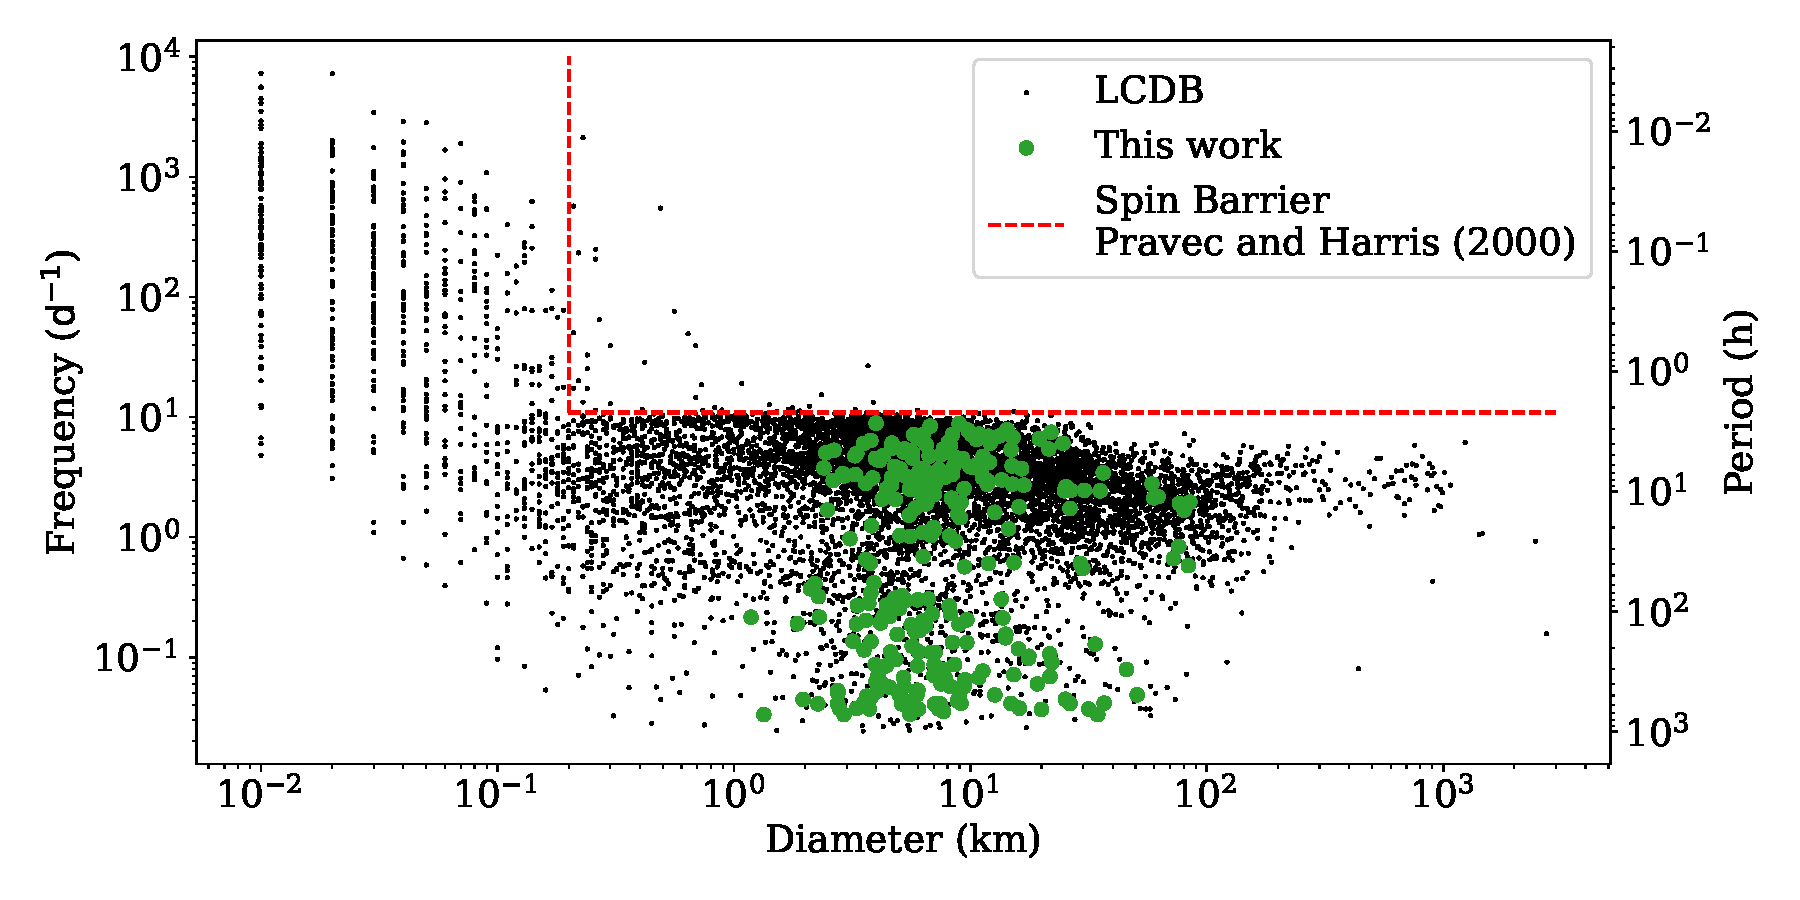
\includegraphics[width=\textwidth]{./Figures/Diam-FreqPlotThisWork.pdf}
  \caption{This work's addition to \autoref{Fig:FreqVsDiam} and the LCDB of \citet{Warner2009}. The diameters are from NEOWISE where available.}
  \label{Fig:FreqDiamUpdate}
\end{figure}

\autoref{Fig:FreqDiamUpdate} shows how my rotation periods fit with those in the LCDB of \cite{Warner2009} from \autoref{Fig:FreqVsDiam}.
It is clear that TESS struggles to determine periods for asteroids with a diameter $\lesssim \qty{1}{\kilo \metre}$. 
This is most likely due to these bodies being too dim for the telescope.  
The spin barrier of \citet{Pravec2000} is not violated by any of the periods I have calculated.

269 of the asteroids that pass the quality checks have diameters in the near-Earth object wide-field infrared survey explorer (NEOWISE) V2.0 database \citep{Masiero2011, NEOWISE2019}.
It is only this sub-sample of the 374 asteroids that are plotted in \autoref{Fig:FreqDiamUpdate}.
The diameters in the LCBD are not calculated using NEOWISE data, so there could be discrepancies in those asteroids that I have calculated periods for that are also in the LCDB. 
The NEOWISE data is self-consistent and encompasses more asteroids that the diameters from just the LCDB, so it was preferred for the over plotting of the rotation data from this work.



\begin{figure}
  \centering
  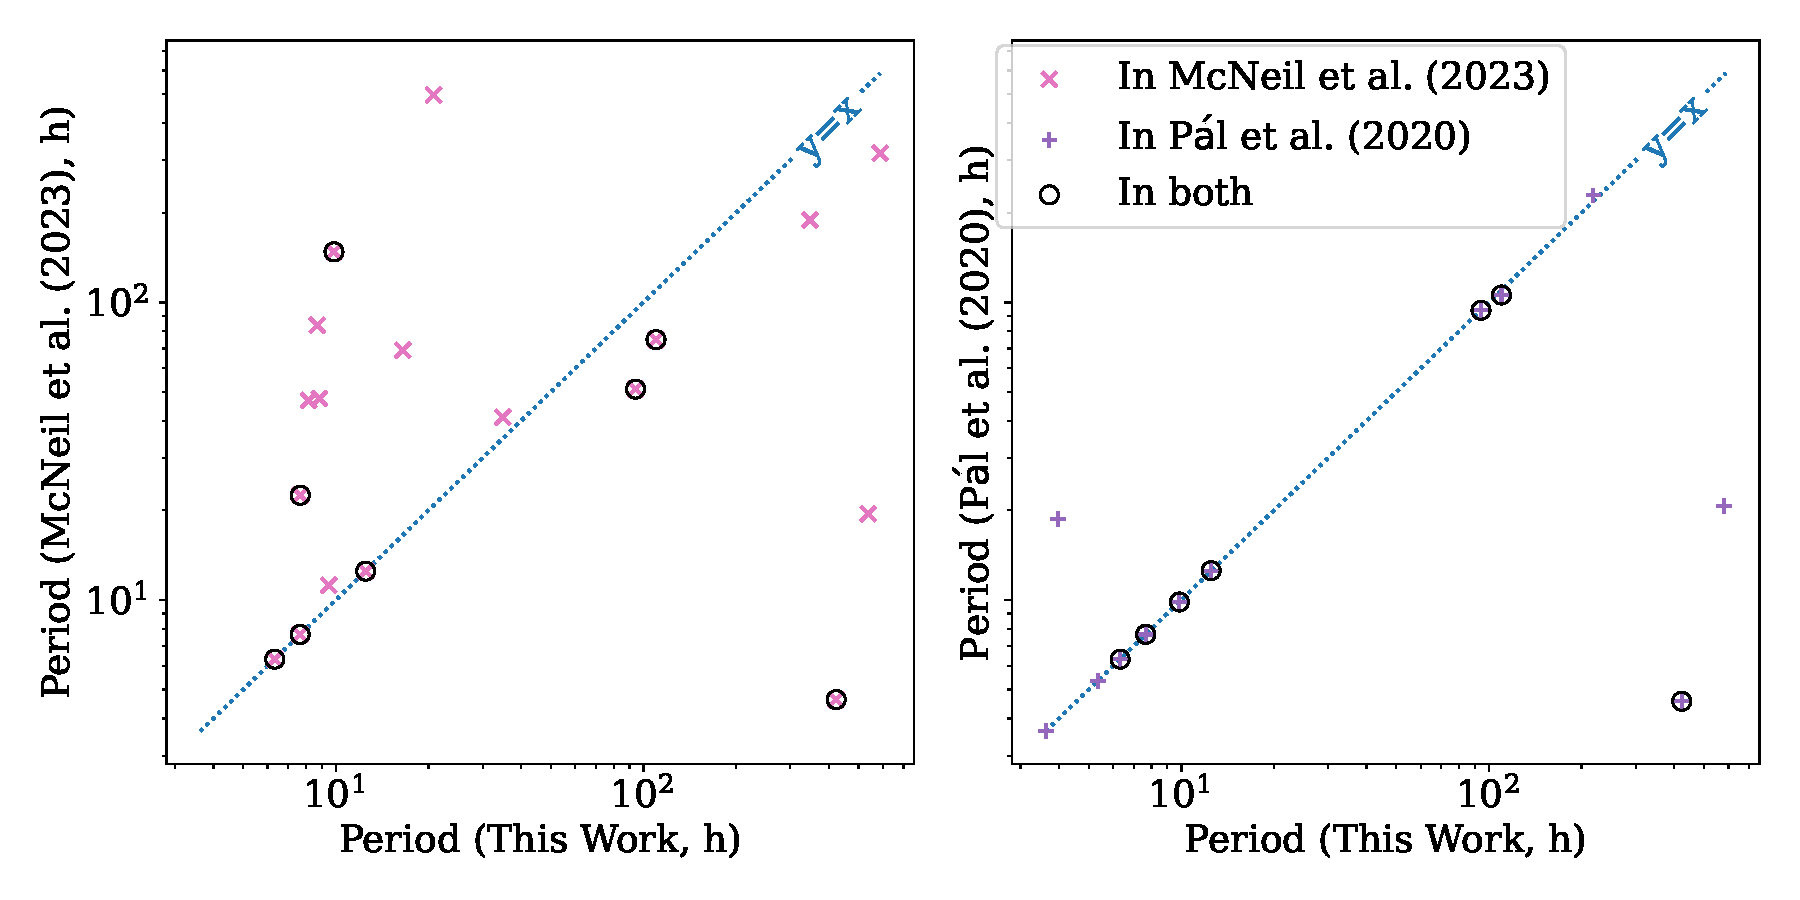
\includegraphics[width=\textwidth]{./Figures/M23andP20Comp.pdf}
  \caption[Comparison to periods from other work]{Comparison of the rotation periods I have calculated to the publicly available data from \citet{McNeill2023} (left, pink crosses) and \citet{Pal2020} (right, purple pluses). The asteroids that are in all three are highlighted with black rings around the symbols.}
\end{figure}

18 in \citet{McNeill2023}
13 in \citet{Pal2020}



The limiting magnitude of the recovery fraction demonstrated in \autoref{Fig:RecovPassorFail} agrees well with other tests of \texttt{TESSELLATE}.
Concurrent work by another Honours' student \citep{MontillaHons} achieves a similar recovery fraction detection efficiency of $\sim$\nth{17} \unit{\mag}.
They have been preforming injection/recovery tests across many TESS sectors, and they find that the limiting magnitude is consistent across sectors
The cadence of the FFIs also seems to have no effect on the depth of the images.
This is promising, as it means that asteroids will be detected to a similar depth as they are here for any further sectors processed, something I could not check myself.

\subsection{Future work}

%quality checks aren't great
It is clear from the outliers in \autoref{Fig:perVSamp} and the clearly incorrect periods of know objects in \autoref{Fig:LCDBcomp} that the quality checks have room for improvement.
Some of these checks were  taken to agree with the how others analyse similar data, like the maximum period from \citet{McNeill2023}.
Others were more empherically derived, such as the minimum average flux value.
There is a delecate balance between detecting as many known periods as possible and maintating strict enough cuts to keep out the junk.

The periodogram noise at the low frequency end is quite strong throughout the range of rotation periods.
Currently, it is responsible for a lot of undetected rotation rates, due to the \qty{90}{\percent} of the \qty{17}{\day} window check, and this noise region having a larger power than any signal.
Modelling this excess to try and remove the noise and boost the signal from the rotation could be done to improve the maximum power of the periodogram.
There are a few asteroids with known longer rotation periods than this check allows for, but one TESS sector will not be enough to determine those accurately.

Linking lightcurves of asteroids between sectors was not considered here, as only one sector has been analysed.
An asteroid will be in multiple sectors, as TESS has surveyed that whole sky more than once.
The different FFI cadence, as well as the large temporal gap between these observations makes it non-trivial to recover the rotation periods.
One could calculate the rotation period in each sector, and then average.
This technique once again biases against long rotation periods, which combining sectors should help with, not hinder.

Lomb-Scargle periodograms can deal with large gaps in the time data, but would require the flux values to have the same normilisation.
\texttt{TESSELLATE} is self consistent in the data reduction for a sector, but comparing fluxes between sectors may have some difficulties.
Assuming the mean flux of the asteroid should be constant, subtracting the mean and 

There are also phase and viewing angle effects on the lightcurve that are important to correct for with large time gaps. 
These were not considered for the single sector analysis because 






%run on rest of TESSELLATE data

\section{Conclusion}\label{Sec:Conc}

It works ok

but could be better

summerise findings

\newpage %* Page number above here must be <=25

\section*{Acknowledgements}
\addcontentsline{toc}{section}{Acknowledgements}
%OzSTAR asks for:
\small
This work was performed on the OzSTAR national facility at Swinburne University of Technology.
The OzSTAR program receives funding in part from the Astronomy National Collaborative Research Infrastructure Strategy (NCRIS) allocation provided by the Australian Government, and from the Victorian Higher Education State Investment Fund (VHESIF) provided by the Victorian Government.

This research has made use of data and/or services provided by the International Astronomical Union's Minor Planet Center.

This work has used data and/or services provided by NASA's Solar System Dynamics website, \url{https://ssd.jpl.nasa.gov/}. Specifically \texttt{JPL Horizons}: \url{https://ssd.jpl.nasa.gov/horizons/}.

The figures seen in this work have been plotted by \texttt{Matplotlib} \citep{Hunter2007}, specifically Version 3.9.2 \citep{PLT3.9.2}

This research made use of Photutils, an Astropy package for detection and photometry of astronomical sources \citep{Bradley2024}.

%*Bib
\addcontentsline{toc}{section}{References}
% \bibliographystyle{jphysicsB}
\bibliography{bibfile.bib}
\end{document}



